% Options for packages loaded elsewhere
\PassOptionsToPackage{unicode}{hyperref}
\PassOptionsToPackage{hyphens}{url}
%
\documentclass[
  ignorenonframetext,
  aspectratio=169,
  t]{beamer}
\usepackage{pgfpages}
\setbeamertemplate{caption}[numbered]
\setbeamertemplate{caption label separator}{: }
\setbeamercolor{caption name}{fg=normal text.fg}
\beamertemplatenavigationsymbolsempty
% Prevent slide breaks in the middle of a paragraph
\widowpenalties 1 10000
\raggedbottom

\usepackage{amsmath,amssymb}
\usepackage{iftex}
\ifPDFTeX
  \usepackage[T1]{fontenc}
  \usepackage[utf8]{inputenc}
  \usepackage{textcomp} % provide euro and other symbols
\else % if luatex or xetex
  \usepackage{unicode-math}
  \defaultfontfeatures{Scale=MatchLowercase}
  \defaultfontfeatures[\rmfamily]{Ligatures=TeX,Scale=1}
\fi
\usepackage{lmodern}
\ifPDFTeX\else  
    % xetex/luatex font selection
\fi
% Use upquote if available, for straight quotes in verbatim environments
\IfFileExists{upquote.sty}{\usepackage{upquote}}{}
\IfFileExists{microtype.sty}{% use microtype if available
  \usepackage[]{microtype}
  \UseMicrotypeSet[protrusion]{basicmath} % disable protrusion for tt fonts
}{}
\makeatletter
\@ifundefined{KOMAClassName}{% if non-KOMA class
  \IfFileExists{parskip.sty}{%
    \usepackage{parskip}
  }{% else
    \setlength{\parindent}{0pt}
    \setlength{\parskip}{6pt plus 2pt minus 1pt}}
}{% if KOMA class
  \KOMAoptions{parskip=half}}
\makeatother
\usepackage{xcolor}
\newif\ifbibliography
\setlength{\emergencystretch}{3em} % prevent overfull lines
\setcounter{secnumdepth}{-\maxdimen} % remove section numbering

\usepackage{color}
\usepackage{fancyvrb}
\newcommand{\VerbBar}{|}
\newcommand{\VERB}{\Verb[commandchars=\\\{\}]}
\DefineVerbatimEnvironment{Highlighting}{Verbatim}{commandchars=\\\{\}}
% Add ',fontsize=\small' for more characters per line
\usepackage{framed}
\definecolor{shadecolor}{RGB}{241,243,245}
\newenvironment{Shaded}{\begin{snugshade}}{\end{snugshade}}
\newcommand{\AlertTok}[1]{\textcolor[rgb]{0.68,0.00,0.00}{#1}}
\newcommand{\AnnotationTok}[1]{\textcolor[rgb]{0.37,0.37,0.37}{#1}}
\newcommand{\AttributeTok}[1]{\textcolor[rgb]{0.40,0.45,0.13}{#1}}
\newcommand{\BaseNTok}[1]{\textcolor[rgb]{0.68,0.00,0.00}{#1}}
\newcommand{\BuiltInTok}[1]{\textcolor[rgb]{0.00,0.23,0.31}{#1}}
\newcommand{\CharTok}[1]{\textcolor[rgb]{0.13,0.47,0.30}{#1}}
\newcommand{\CommentTok}[1]{\textcolor[rgb]{0.37,0.37,0.37}{#1}}
\newcommand{\CommentVarTok}[1]{\textcolor[rgb]{0.37,0.37,0.37}{\textit{#1}}}
\newcommand{\ConstantTok}[1]{\textcolor[rgb]{0.56,0.35,0.01}{#1}}
\newcommand{\ControlFlowTok}[1]{\textcolor[rgb]{0.00,0.23,0.31}{#1}}
\newcommand{\DataTypeTok}[1]{\textcolor[rgb]{0.68,0.00,0.00}{#1}}
\newcommand{\DecValTok}[1]{\textcolor[rgb]{0.68,0.00,0.00}{#1}}
\newcommand{\DocumentationTok}[1]{\textcolor[rgb]{0.37,0.37,0.37}{\textit{#1}}}
\newcommand{\ErrorTok}[1]{\textcolor[rgb]{0.68,0.00,0.00}{#1}}
\newcommand{\ExtensionTok}[1]{\textcolor[rgb]{0.00,0.23,0.31}{#1}}
\newcommand{\FloatTok}[1]{\textcolor[rgb]{0.68,0.00,0.00}{#1}}
\newcommand{\FunctionTok}[1]{\textcolor[rgb]{0.28,0.35,0.67}{#1}}
\newcommand{\ImportTok}[1]{\textcolor[rgb]{0.00,0.46,0.62}{#1}}
\newcommand{\InformationTok}[1]{\textcolor[rgb]{0.37,0.37,0.37}{#1}}
\newcommand{\KeywordTok}[1]{\textcolor[rgb]{0.00,0.23,0.31}{#1}}
\newcommand{\NormalTok}[1]{\textcolor[rgb]{0.00,0.23,0.31}{#1}}
\newcommand{\OperatorTok}[1]{\textcolor[rgb]{0.37,0.37,0.37}{#1}}
\newcommand{\OtherTok}[1]{\textcolor[rgb]{0.00,0.23,0.31}{#1}}
\newcommand{\PreprocessorTok}[1]{\textcolor[rgb]{0.68,0.00,0.00}{#1}}
\newcommand{\RegionMarkerTok}[1]{\textcolor[rgb]{0.00,0.23,0.31}{#1}}
\newcommand{\SpecialCharTok}[1]{\textcolor[rgb]{0.37,0.37,0.37}{#1}}
\newcommand{\SpecialStringTok}[1]{\textcolor[rgb]{0.13,0.47,0.30}{#1}}
\newcommand{\StringTok}[1]{\textcolor[rgb]{0.13,0.47,0.30}{#1}}
\newcommand{\VariableTok}[1]{\textcolor[rgb]{0.07,0.07,0.07}{#1}}
\newcommand{\VerbatimStringTok}[1]{\textcolor[rgb]{0.13,0.47,0.30}{#1}}
\newcommand{\WarningTok}[1]{\textcolor[rgb]{0.37,0.37,0.37}{\textit{#1}}}

\providecommand{\tightlist}{%
  \setlength{\itemsep}{0pt}\setlength{\parskip}{0pt}}\usepackage{longtable,booktabs,array}
\usepackage{calc} % for calculating minipage widths
\usepackage{caption}
% Make caption package work with longtable
\makeatletter
\def\fnum@table{\tablename~\thetable}
\makeatother
\usepackage{graphicx}
\makeatletter
\def\maxwidth{\ifdim\Gin@nat@width>\linewidth\linewidth\else\Gin@nat@width\fi}
\def\maxheight{\ifdim\Gin@nat@height>\textheight\textheight\else\Gin@nat@height\fi}
\makeatother
% Scale images if necessary, so that they will not overflow the page
% margins by default, and it is still possible to overwrite the defaults
% using explicit options in \includegraphics[width, height, ...]{}
\setkeys{Gin}{width=\maxwidth,height=\maxheight,keepaspectratio}
% Set default figure placement to htbp
\makeatletter
\def\fps@figure{htbp}
\makeatother
% definitions for citeproc citations
\NewDocumentCommand\citeproctext{}{}
\NewDocumentCommand\citeproc{mm}{%
  \begingroup\def\citeproctext{#2}\cite{#1}\endgroup}
\makeatletter
 % allow citations to break across lines
 \let\@cite@ofmt\@firstofone
 % avoid brackets around text for \cite:
 \def\@biblabel#1{}
 \def\@cite#1#2{{#1\if@tempswa , #2\fi}}
\makeatother
\newlength{\cslhangindent}
\setlength{\cslhangindent}{1.5em}
\newlength{\csllabelwidth}
\setlength{\csllabelwidth}{3em}
\newenvironment{CSLReferences}[2] % #1 hanging-indent, #2 entry-spacing
 {\begin{list}{}{%
  \setlength{\itemindent}{0pt}
  \setlength{\leftmargin}{0pt}
  \setlength{\parsep}{0pt}
  % turn on hanging indent if param 1 is 1
  \ifodd #1
   \setlength{\leftmargin}{\cslhangindent}
   \setlength{\itemindent}{-1\cslhangindent}
  \fi
  % set entry spacing
  \setlength{\itemsep}{#2\baselineskip}}}
 {\end{list}}
\usepackage{calc}
\newcommand{\CSLBlock}[1]{\hfill\break\parbox[t]{\linewidth}{\strut\ignorespaces#1\strut}}
\newcommand{\CSLLeftMargin}[1]{\parbox[t]{\csllabelwidth}{\strut#1\strut}}
\newcommand{\CSLRightInline}[1]{\parbox[t]{\linewidth - \csllabelwidth}{\strut#1\strut}}
\newcommand{\CSLIndent}[1]{\hspace{\cslhangindent}#1}

%\usepackage[round,authoryear]{natbib}
\usepackage{paralist}
\usepackage{pgfpages}
\usepackage{mathtools}
\usepackage{amsmath}
\usepackage{amssymb}
\usepackage{xspace}        
\usepackage{graphicx}

\usepackage{amsthm}
\theoremstyle{definition}
\newtheorem{thm}{Theorem}
\newtheorem{exercise}{Exercise}
\newtheorem{challenge}{Challenge}

\bibliographystyle{jss}

\newcommand\prob[1]{\mathbb{P}\left[{#1}\right]}
\newcommand\expect[1]{\mathbb{E}\left[{#1}\right]}
\newcommand\var[1]{\mathrm{Var}\left[{#1}\right]}
\newcommand\dist[2]{\mathrm{#1}\left(#2\right)}
\newcommand\lik{\mathcal{L}}
\newcommand\loglik{\ell}
\newcommand\R{\mathbb{R}}
\newcommand\Rzero{\mathfrak{R}_0}
\newcommand\argmax{\mathop{\mathrm{argmax}}}
\newcommand\argmin{\mathop{\mathrm{argmin}}}

\newcommand\code[1]{\texttt{#1}}
\newcommand\pkg[1]{\textbf{#1}}

\newcommand\link[2]{\href{#1}{#2}}
\newcommand{\doi}[1]{\link{https://doi.org/#1}{\texttt{doi:~{#1}}}}

\newcommand{\scinot}[2]{#1{\times}10^{#2}}
\newcommand{\dd}[1]{\mathrm{d}{#1}}
\newcommand{\pd}[3][]{%
  \def\ord{#1} \ifx\ord\empty%
  \frac{\partial{#2}}{\partial{#3}}%
  \else \frac{\partial^{#1}{#2}}{\partial{#3}^{#1}}%
  \fi
}
\newcommand{\deriv}[3][]{%
  \def\ord{#1} \ifx\ord\empty%
  \frac{\dd{#2}}{\dd{#3}}%
  \else \frac{\dd^{#1}{#2}}{\dd{#3}^{#1}}%
  \fi
}

\newcommand\Rlanguage{\textsf{R}\xspace}

\newcounter{Ecounter}
\newcommand\myexercise{{\stepcounter{Ecounter} Exercise \CHAPTER.\theEcounter}}

\newcommand\myexample{{\bf Example}}
\newcommand\mydot{{\,\cdot\,}}
\newcommand\myref[1]{\m{#1}}

\newcommand\Rspace{\mathcal{R}}

\renewcommand\vec[1]{\boldsymbol{\mathrm{#1}}}
\newcommand\vect[1]{\vec{#1}}
\newcommand\mat[1]{\mathbb{#1}}
\newcommand\pr{\mathbb{P}}
\newcommand\E{\mathbb{E}}

\newcommand\profileloglik[1]{\ell^\mathrm{profile}_#1}
\newcommand\Real{\mathbb{R}}

\newcommand\bi{\begin{itemize}}
\newcommand\ei{\end{itemize}}

\newcommand\normal{\mathrm{Normal}}

\newcommand\iid{\mathrm{iid}}
\newcommand\MVN{\mathrm{MVN}}
\newcommand\SE{\mathrm{SE}}

\newcommand\pval{\mathrm{pval}}
% \newcommand\var{\mathrm{Var}}
\newcommand\sd{\mathrm{SD}}
\newcommand\sdSample{\mathrm{sd}}
\newcommand\varSample{\mathrm{var}}
\newcommand\cov{\mathrm{Cov}}
\newcommand\covSample{\mathrm{cov}}
\newcommand\corSample{\mathrm{cor}}
\newcommand\cor{\mathrm{Cor}}
\newcommand\given{{\, | \,}}
\newcommand\param{\,;}
\newcommand\params{\param}
\newcommand\equals{{ \, = \, }}
\newcommand\myemph[1]{{\textbf{#1}}}

\setlength{\parskip}{0mm}
\setlength{\parindent}{0mm}
\makeatletter
\@ifpackageloaded{caption}{}{\usepackage{caption}}
\AtBeginDocument{%
\ifdefined\contentsname
  \renewcommand*\contentsname{Table of contents}
\else
  \newcommand\contentsname{Table of contents}
\fi
\ifdefined\listfigurename
  \renewcommand*\listfigurename{List of Figures}
\else
  \newcommand\listfigurename{List of Figures}
\fi
\ifdefined\listtablename
  \renewcommand*\listtablename{List of Tables}
\else
  \newcommand\listtablename{List of Tables}
\fi
\ifdefined\figurename
  \renewcommand*\figurename{Figure}
\else
  \newcommand\figurename{Figure}
\fi
\ifdefined\tablename
  \renewcommand*\tablename{Table}
\else
  \newcommand\tablename{Table}
\fi
}
\@ifpackageloaded{float}{}{\usepackage{float}}
\floatstyle{ruled}
\@ifundefined{c@chapter}{\newfloat{codelisting}{h}{lop}}{\newfloat{codelisting}{h}{lop}[chapter]}
\floatname{codelisting}{Listing}
\newcommand*\listoflistings{\listof{codelisting}{List of Listings}}
\makeatother
\makeatletter
\makeatother
\makeatletter
\@ifpackageloaded{caption}{}{\usepackage{caption}}
\@ifpackageloaded{subcaption}{}{\usepackage{subcaption}}
\makeatother
\ifLuaTeX
  \usepackage{selnolig}  % disable illegal ligatures
\fi
\usepackage{bookmark}

\IfFileExists{xurl.sty}{\usepackage{xurl}}{} % add URL line breaks if available
\urlstyle{same} % disable monospaced font for URLs
\hypersetup{
  pdftitle={Lesson 2: Simulation of stochastic dynamic models},
  pdfauthor={Qianying (Ruby) Lin; Spencer J. Fox; Zian (Larry) Zhuang},
  hidelinks,
  pdfcreator={LaTeX via pandoc}}

\title{Lesson 2: Simulation of stochastic dynamic models}
\author{Qianying (Ruby) Lin \and Spencer J. Fox \and Zian (Larry)
Zhuang}
\date{}

\begin{document}
\frame{\titlepage}

\begin{frame}{Objectives}
\phantomsection\label{objectives}
This tutorial develops some classes of dynamic models relevant to
biological systems, especially for epidemiology.

\begin{enumerate}
\tightlist
\item
  Dynamic systems can often be represented in terms of \emph{flows}
  between \emph{compartments}.
\item
  We develop the concept of a \emph{compartment model} for which we
  specify \emph{rates} for the flows between compartments.
\item
  We show how deterministic and stochastic versions of a compartment
  model are derived and related.
\item
  We introduce Euler's method to simulate from dynamic models.
\item
  We specify deterministic and stochastic compartment models in pomp
  using Euler method simulation.
\end{enumerate}
\end{frame}

\section{Compartmental models}\label{compartmental-models}

\section{Example: the SIR model}\label{example-the-sir-model}

\begin{frame}[allowframebreaks]{A basic compartment model: The SIR
model}
\phantomsection\label{a-basic-compartment-model-the-sir-model}
\begin{itemize}
\item
  We develop deterministic and stochastic representations of a
  susceptible-infected-recovered (SIR) system, a fundamental class of
  models for disease transmission dynamics.
\item
  We set up notation applicable to general compartment models (Bretó et
  al. 2009). %%%%% SIR diagram
\begin{center}
  \resizebox{0.65\textwidth}{!}{
    \Large
    \setlength{\unitlength}{5pt}
    \begin{picture}(44,20)(-5,-4)
      \thicklines
      \put(0,0){\framebox(6,6){S}}
      \put(16,0){\framebox(6,6){I}}
      \put(32,0){\framebox(6,6){R}}
      \put(-5,3){\vector(1,0){4}}
      \put(-5,0){$\mu^{}_{BS}$}
      \put(6,3){\vector(1,0){10}}
      \put(9,0){$\mu_{SI}^{}$}
      \put(11,4){\vector(0,1){5}}
      \put(11.7,6){$\rho$}
      \put(11,11.5){\circle{5}}
      \put(9.8,10.6){{$C$}}
      \put(3,-0.2){\vector(0,-1){4}}
      \put(4,-3){$\mu^{}_{SD}$}
      \put(19,-0.2){\vector(0,-1){4}}
      \put(20,-3){$\mu^{}_{ID}$}
      \put(22,3){\vector(1,0){10}}
      \put(26,0){$\mu_{IR}^{}$}
      \put(35,-0.2){\vector(0,-1){4}}
      \put(36,-3){$\mu_{RD}^{}$}
    \end{picture}
  }
\end{center}
 \vspace{5mm}

  \begin{tabular}{c @{\ :\ } l c @{\ :\ } l}
    S & susceptible & I & infected and infectious  \\
    R & recovered and/or removed  & C & reported cases
  \end{tabular}
\item
  We suppose that each arrow has an associated rate, so here there is a
  rate \(\mu_{SI}(t)\) at which individuals in \(S\) transition to
  \(I\), and \(\mu_{IR}\) at which individuals in \(I\) transition to
  \(R\).
\item
  To account for demography (births/deaths/migration) we allow the
  possibility of a source and sink compartment, which is not usually
  represented on the flow diagram. We write \(\mu_{BS}\) for a rate of
  births into \(S\), and denote mortality rates by \(\mu_{SD}\),
  \(\mu_{ID}\), \(\mu_{RD}\).
\item
  The rates may be either constant or time-varying.
\item
  For the simplest SIR model, ignoring demography, we set
  \[ \mu_{BS}=\mu_{SD}=\mu_{ID}=\mu_{RD}=0.\]
\end{itemize}
\end{frame}

\section{Notation}\label{notation}

\begin{frame}[allowframebreaks]{General notation for compartment models}
\phantomsection\label{general-notation-for-compartment-models}
To develop a systematic notation, it turns out to be convenient to keep
track of the flows between compartments as well as the number of
individuals in each compartment:

\begin{itemize}
\item
  \(N_{SI}(t)\): the number of individuals who have transitioned from
  \(S\) to \(I\) \textbf{by} time \(t\). We say that \(N_{SI}(t)\) is a
  \emph{counting process}.
\item
  \(N_{IR}(t)\): the number of individuals transitioning from \(I\) to
  \(R\) \textbf{by} time \(t\).
\end{itemize}

To include demography, we could keep track of birth and death events by
the counting processes:

\begin{itemize}
\item
  \(N_{BS}(t)\): the number of newborns into \(S\) \textbf{by} time
  \(t\).
\item
  \(N_{SD}(t)\), \(N_{ID}(t)\), \(N_{RD}(t)\): the number of deaths from
  \(S\), \(I\), and \(R\) compartments \textbf{by} time \(t\),
  respectively.
\end{itemize}

\framebreak

\begin{itemize}
\tightlist
\item
  For discrete population compartment models, the flow counting
  processes are non-decreasing and integer valued.
\item
  For continuous population compartment models, the flow counting
  processes are non-decreasing and real valued.
\end{itemize}
\end{frame}

\begin{frame}{Compartment model from counting processes}
\phantomsection\label{compartment-model-from-counting-processes}
\begin{itemize}
\item
  The numbers of people in each compartment can be computed via these
  counting processes. Ignoring demography, we have: \begin{equation*}
   \begin{aligned}
     S(t) &= S(0) - N_{SI}(t) &\\
     I(t) &= I(0) + N_{SI}(t) &- N_{IR}(t) \\
     R(t) &= R(0) &+ N_{IR}(t)
   \end{aligned}
      \end{equation*}
\item
  These equations represent \emph{conservation of individuals} or
  \emph{what goes in must come out}.
\end{itemize}
\end{frame}

\begin{frame}{Ordinary differential equation interpretation}
\phantomsection\label{ordinary-differential-equation-interpretation}
Together with initial conditions specifying \(S(0)\), \(I(0)\) and
\(R(0)\), we just need to write down ordinary differential equations
(ODEs) for the flow counting processes. These are: \begin{equation*}
    \begin{aligned}
      \deriv{N_{SI}}{t} &= \mu_{SI}(t)\,S(t)\\
      \deriv{N_{IR}}{t} &= \mu_{IR}\,I(t)
    \end{aligned}
  \end{equation*}
\end{frame}

\begin{frame}{Common notation for a deterministic SIR model}
\phantomsection\label{common-notation-for-a-deterministic-sir-model}
\begin{center}
    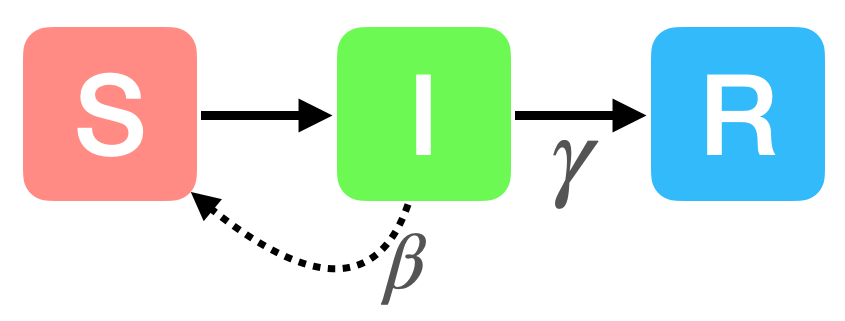
\includegraphics[height=3cm]{../graphics/simple-sir.png}
\end{center}

\begin{itemize}
\tightlist
\item
  \(\beta\): transmission rate, encompasses the frequency of contacts
  and transmission probability between individuals
\item
  \(\gamma\): recovery rate, rate that infected individuals become
  ``uninfectious''

  \begin{itemize}
  \tightlist
  \item
    Duration of infectiousness on average is \(\frac{1}{\gamma}\)
  \end{itemize}
\item
  \(S + I + R = N\)
\end{itemize}
\end{frame}

\begin{frame}{Common notation for a deterministic SIR model - equations}
\phantomsection\label{common-notation-for-a-deterministic-sir-model---equations}
\begin{center}
    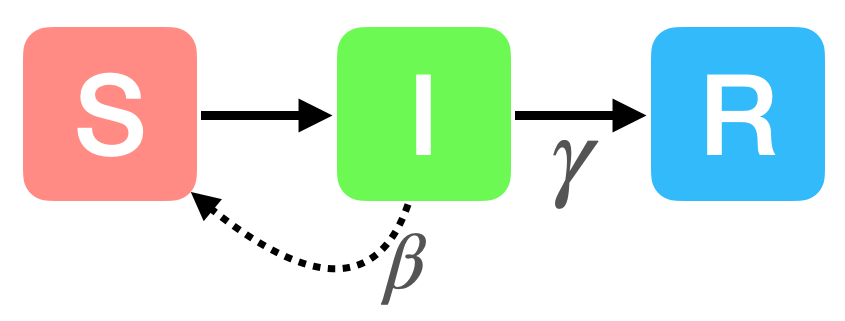
\includegraphics[height=3cm]{../graphics/simple-sir.png}
\end{center}

\begin{equation*}
\begin{aligned}
  \deriv{S}{t} &= - \beta S \frac{I}{N}\\
  \deriv{I}{t} &= \beta S \frac{I}{N} - \gamma * I \\
  \deriv{R}{t} &= \gamma I
\end{aligned}
\end{equation*}
\end{frame}

\begin{frame}[fragile]{Common notation for a deterministic SIR model -
Skeleton code}
\phantomsection\label{common-notation-for-a-deterministic-sir-model---skeleton-code}
\begin{center}
    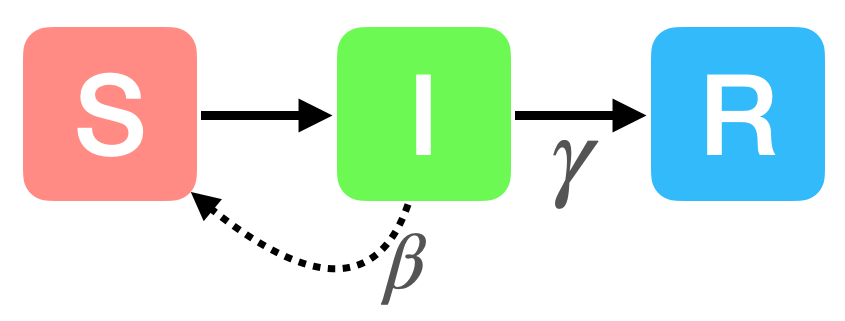
\includegraphics[height=3cm]{../graphics/simple-sir.png}
\end{center}

\begin{columns}[T]
\begin{column}{0.4\textwidth}
\begin{equation*}
\begin{aligned}
  \deriv{S}{t} &= - \beta S \frac{I}{N}\\
  \deriv{I}{t} &= \beta S \frac{I}{N} - \gamma * I \\
  \deriv{R}{t} &= \gamma I
\end{aligned}
\end{equation*}
\end{column}

\begin{column}{0.6\textwidth}
\begin{Shaded}
\begin{Highlighting}[]
\FunctionTok{library}\NormalTok{(pomp)}
\FunctionTok{Csnippet}\NormalTok{(}\StringTok{"}
\StringTok{        DS = {-}Beta*S*I/N;}
\StringTok{        DI = Beta*S*I/N {-} I*Gamma;}
\StringTok{        DR = I*Gamma;}
\StringTok{        "}\NormalTok{) }\OtherTok{{-}\textgreater{}}\NormalTok{ sir\_det\_skel}
\end{Highlighting}
\end{Shaded}
\end{column}
\end{columns}
\end{frame}

\begin{frame}{Spencer component done\ldots{}}
\phantomsection\label{spencer-component-done}
\end{frame}

\section{Stochastic simulations}\label{stochastic-simulations}

\begin{frame}{Stochastic Differential Equations (SDEs)}
\phantomsection\label{stochastic-differential-equations-sdes}
\begin{itemize}
\item
  By including randomness in the ODE system, we can have the stochastic
  differential equation (SDE) system.
\item
  For example, for the ODE \(\deriv{x}{t}=h(x)\), a natural way to add
  stochastic variation is \[
      \deriv{X}{t} = h(X)+\sigma\,\deriv{B}{t}
    \] where \(\{B(t)\}\) is Brownian motion and so \(dB/dt\) is
  Brownian noise.
\end{itemize}
\end{frame}

\begin{frame}[allowframebreaks]{The simple counting process and the
reactions}
\phantomsection\label{the-simple-counting-process-and-the-reactions}
\begin{itemize}
\item
  A deterministic SIR model has a fixed trajectory, indicating that the
  number of each compartment at any time is fixed with given parameters
  and intial states; thus the transitions between compartments are fixed
  at any time.
\item
  A stochastic SIR model, in the contrary, the trajectory and the
  transitions between compartments at any time are stochastic.
\item
  Recall \(N_{SI}(t)\) and \(N_{IR}(t)\) are counting processes,
  indicating the number of total individuals transitioned from \(S\) to
  \(I\) and \(I\) to \(R\) by time \(t\), respectively.
\item
  A \emph{simple counting process} is one which cannot count more than
  one event at a time.
\end{itemize}

\framebreak

\begin{itemize}
\item
  We then can relate the counting process to the common SIR reactions
  with the corresponding probabilities.
\item
  Note that we are using
  \href{./exercises.html\#exercise-little-o-notation}{\emph{little o
  notation}} and we write \(h(\delta)=o(\delta)\) to mean
  \(\lim_{\delta\to 0} \frac{h(\delta)}{\delta} = 0\).
\end{itemize}

\begin{longtable}[]{@{}
  >{\raggedright\arraybackslash}p{(\columnwidth - 4\tabcolsep) * \real{0.3981}}
  >{\raggedright\arraybackslash}p{(\columnwidth - 4\tabcolsep) * \real{0.1553}}
  >{\raggedright\arraybackslash}p{(\columnwidth - 4\tabcolsep) * \real{0.4466}}@{}}
\caption{Relationship between the counting processes, the reactions, and
the probabilities.}\label{tbl-stochproc}\tabularnewline
\toprule\noalign{}
\begin{minipage}[b]{\linewidth}\raggedright
Counting
\end{minipage} & \begin{minipage}[b]{\linewidth}\raggedright
Reaction
\end{minipage} & \begin{minipage}[b]{\linewidth}\raggedright
Probability
\end{minipage} \\
\midrule\noalign{}
\endfirsthead
\toprule\noalign{}
\begin{minipage}[b]{\linewidth}\raggedright
Counting
\end{minipage} & \begin{minipage}[b]{\linewidth}\raggedright
Reaction
\end{minipage} & \begin{minipage}[b]{\linewidth}\raggedright
Probability
\end{minipage} \\
\midrule\noalign{}
\endhead
\(N_{SI}(t+\delta) = N_{SI}(t) + 1\) & \(S \to S - 1\) &
\(\beta S(t) I(t) \delta / N + o(\delta)\) \\
& \(I \to I + 1\) & \\
\(N_{SI}(t+\delta) = N_{SI}(t)\) & &
\(1-\beta S(t) I(t) \delta / N + o(\delta)\) \\
\(N_{IR}(t+\delta) = N_{IR}(t) + 1\) & \(I \to I - 1\) &
\(\gamma I(t) \delta + o(\delta)\) \\
& \(R \to R + 1\) & \\
\(N_{IR}(t+\delta) = N_{IR}(t)\) & &
\(1 - \gamma I(t) \delta + o(\delta)\) \\
\bottomrule\noalign{}
\end{longtable}
\end{frame}

\begin{frame}[allowframebreaks]{The Euler's method}
\phantomsection\label{the-eulers-method}
\begin{itemize}
\tightlist
\item
  When referring the counting and its corresponding probability in
  Table~\ref{tbl-stochproc}, it is obvious that we can derive a
  continuous time Markov chain (CTMC) for the SIR model:
\end{itemize}

\[
     \begin{aligned}
       \pr\big[N_{SI}(t+\delta)&\equals N_{SI}(t)+1\big] &\equals& \beta \, S(t)\, I(t) / N\, \delta + o(\delta),
       \\
       \pr\big[N_{IR}(t+\delta)&\equals N_{IR}(t)+1\big] &\equals& \gamma \, I(t) \delta + o(\delta).
     \end{aligned}
\]

\begin{itemize}
\tightlist
\item
  For \(k=1,2,...\), by discretizing this CTMC with small time step
  \(\delta\), we can derive a numerical solution with the state
  variables \(\tilde S(k\delta)\), \(\tilde I(k\delta)\),
  \(\tilde R(k\delta)\):
\end{itemize}

\[\begin{array}{lcl}
        \tilde S(k\delta)&=& S(0) - \tilde N_{SI}(k\delta) \\
        \tilde I(k\delta)&=& I(0) + \tilde N_{SI}(k\delta) - \tilde N_{IR}(k\delta) \\
        \tilde R(k\delta) &=& R(0) + \tilde N_{IR}(k\delta)
\end{array}\]

\begin{itemize}
\tightlist
\item
  \(\tilde N_{SI}(t)\) and \(\tilde N_{IR}(t)\): the numerical solutions
  for \(N_{SI}(t)\) and \(N_{IR}(t)\)
\end{itemize}

\framebreak

\begin{itemize}
\item
  Let current \(t=k\delta\), consider the small time interval
  \(t\le \tau \le t+\delta\).
\item
  Assume that the gradients \(\deriv{N_{SI}}{t} = \mu_{SI}(t)\,S(t)\)
  and \(\deriv{N_{IR}}{t} = \mu_{IR}\,I(t)\) are approximately constant
\item
  We can have \(\tilde N_{SI}(t+\delta)\) and
  \(\tilde N_{IR}(t+\delta)\) as:
\end{itemize}

\[
\begin{array}{lcl}
        \tilde N_{SI}(t+ \delta) &=& \tilde N_{SI}(t) + \delta\,\beta\, S(t)\,I(t)\,/ N \\
        \tilde N_{IR}(t + \delta) &=& \tilde N_{IR}(t) + \delta\,\gamma\,I(t) \\
\end{array}
\]

\framebreak

Now we can include stochastic variation in the Euler's method.

\begin{itemize}
\tightlist
\item
  Recall the SDE:
\end{itemize}

\[
  \deriv{X}{t} = h(X)+\sigma\,\deriv{B}{t}
\]

where \(\{B(t)\}\) is Brownian motion and so \(dB/dt\) is Brownian
noise.

\begin{itemize}
\tightlist
\item
  An Euler approximation \(\tilde X(t)\) within the small time interval
  \([t,t+\delta]\) and \(t=k\delta\) for \(k=0,1,2,\dots\) is \[
   \tilde{X}\big( \,t + \delta\,\big) = \tilde{X}(t) + \delta\, h\big(\, \tilde{X}(t)\,\big) + \sigma \sqrt{\delta} \, Z_k
  \]
\end{itemize}

where \(Z_1,Z_2,\dots\) are independent standard normal random
variables, i.e., \(Z_k\sim \dist{Normal}{0,1}\).

\begin{itemize}
\tightlist
\item
  Although SDEs are often considered an advanced topic in probability,
  the Euler approximation doesn't demand much more than familiarity with
  the normal distribution.
\end{itemize}

\framebreak

Now we can consider applying the Euler's method for a stochastic SIR
model:

\begin{itemize}
\tightlist
\item
  A binomial approximation with exponential transition probabilities.
\end{itemize}

\[
\begin{aligned}
        \tilde N_{SI}(t+ \delta) &= \tilde N_{SI}(t) + \mathrm{Binomial}\big[\tilde S(t),1-\exp\big\{-\beta\,\tilde I(t)/ N\,\delta\big\}\big], \\
        \tilde N_{IR}(t + \delta) &= \tilde N_{IR}(t) + \mathrm{Binomial}\big[\tilde I(t), 1-\exp\big\{-\delta\,\gamma\big\}\big], \\
\end{aligned}
\]

where \(\mathrm{Binomial}(n,p)\) is a binomial random variable with mean
\(np\) and variance \(np(1-p)\). Here,
\(p=1-\exp\big\{-\beta\,\tilde I(t)/ N\,\delta\big\}\) and
\(p=1-\exp\big\{-\delta\,\gamma\big\}\), respectively.

\framebreak

The following are two other ways for a stochastic SIR model with the
Euler's approximation, what they are not as good as the previous one?

\begin{enumerate}
\item
  A Poisson approximation.
  \[\tilde N_{SI}(t+\delta)= \tilde N_{SI}(t) + \mathrm{Poisson}\big[\beta\,\tilde S(t)\,\tilde I(t) / N\, \delta\big],\]
  where \(\mathrm{Poisson}(\mu)\) is a Poisson random variable with mean
  \(\mu=\beta\,\tilde S(t)\,\tilde I(t) / N\, \delta\).
\item
  A binomial approximation,
  \[\tilde N_{SI}(t+\delta) = \tilde N_{SI}(t) + \mathrm{Binomial}\big[\tilde S(t),\beta\,\tilde I(t) / N \, \delta\big].\]
\end{enumerate}
\end{frame}

\begin{frame}[allowframebreaks]{The Gillespie method}
\phantomsection\label{the-gillespie-method}
\begin{itemize}
\item
  Numerical methods, such as the Euler's method, are approximations to
  the process by discretizing time using small time step \(\delta\)
\item
  However, the Gillespie method is the exact \textbf{Stochastic
  Simulation Method}, which leverages the Markov Property as well.
\item
  In Table~\ref{tbl-stochproc}, by consider the reactions and the
  probabilities, we can derive the Gillespie algorithm for the
  stochastic SIR model.
\end{itemize}

\framebreak

With initialization, \(S(0)\), \(I(0)\), and \(R(0)\), at current time
\(t\):

\begin{enumerate}
\item
  Compute the total event rates:
  \(\lambda_1 = \beta\,S(t)\,I(t)/N, \lambda_2 = \gamma\,I(t), \lambda = \lambda_1 + \lambda_2\)
\item
  Compute the waiting time
  \(\Delta t \sim \mathrm{Exponential}(\lambda)\)
\item
  Select the reactions by sampling from probabilities
  \(\left(\frac{\lambda_1}{\lambda}, \frac{\lambda_2}{\lambda}\right)\)
\item
  Update the states from the selected reaction and update the time
  \(t\to t+\Delta t\)
\item
  Repeat 1-4 till the end of the simulation time
\end{enumerate}

\vfill

Even though the Gillespie is an exact stochastic simulation method, it
has limitations such as:

\begin{itemize}
\item
  Computational Intensity: For complex systems with many reactions, the
  Gillespie method can become computationally expensive.
\item
  Rare Events: For systems where some reactions are very rare, a large
  number of simulation steps may be needed to capture these events,
  making the method slow.
\end{itemize}
\end{frame}

\begin{frame}{Euler vs.~Gillespie}
\phantomsection\label{euler-vs.-gillespie}
\begin{itemize}
\tightlist
\item
  Why and When would you prefer an implementation of Gillespie's
  algorithm to an Euler solution?
\end{itemize}

\vspace{3mm}

\href{./exercises.html\#exercise-euler-versus-gillespie}{Worked solution
to the Exercise}

\vspace{3mm}

\begin{itemize}
\tightlist
\item
  Numerically, Gillespie's algorithm is often approximated using
  so-called
  \href{https://en.wikipedia.org/wiki/Tau-leaping}{tau-leaping} methods.
  These are closely related to Euler's approach. In this context, the
  Euler method has sometimes been called tau-leaping.
\end{itemize}
\end{frame}

\begin{frame}[fragile,allowframebreaks]{Compartment models in
\texttt{pomp}: The Consett Measles outbreaks}
\phantomsection\label{compartment-models-in-pomp-the-consett-measles-outbreaks}
Let's look at outbreak of measles in the town of Consett in England in
1948:

\begin{itemize}
\item
  the town had population of 38820,
\item
  with 737 births over the course of the year.
\end{itemize}

\begin{Shaded}
\begin{Highlighting}[]
\FunctionTok{library}\NormalTok{(tidyverse)}
\FunctionTok{read\_csv}\NormalTok{(}\FunctionTok{paste0}\NormalTok{(}\StringTok{"https://kingaa.github.io/sbied/stochsim/"}\NormalTok{, }
  \StringTok{"Measles\_Consett\_1948.csv"}\NormalTok{)) }\SpecialCharTok{|\textgreater{}} 
  \FunctionTok{select}\NormalTok{(week,}\AttributeTok{reports=}\NormalTok{cases) }\OtherTok{{-}\textgreater{}}\NormalTok{ meas}
\NormalTok{meas }\SpecialCharTok{|\textgreater{}} \FunctionTok{as.data.frame}\NormalTok{() }\SpecialCharTok{|\textgreater{}} \FunctionTok{head}\NormalTok{(}\AttributeTok{n=}\DecValTok{3}\NormalTok{)}
\end{Highlighting}
\end{Shaded}

\begin{verbatim}
 week reports
    1       0
    2       0
    3       2
\end{verbatim}

\vspace{-25mm}

\begin{columns}[T]
\begin{column}{0.3\textwidth}
\end{column}

\begin{column}{0.7\textwidth}
\begin{itemize}
\item
  \texttt{week}: time, indicates that the data are counted weekly
\item
  \texttt{reports} variable: incidence, counts the number of reports of
  new measles cases each week
\end{itemize}
\end{column}
\end{columns}

\framebreak

\begin{center}
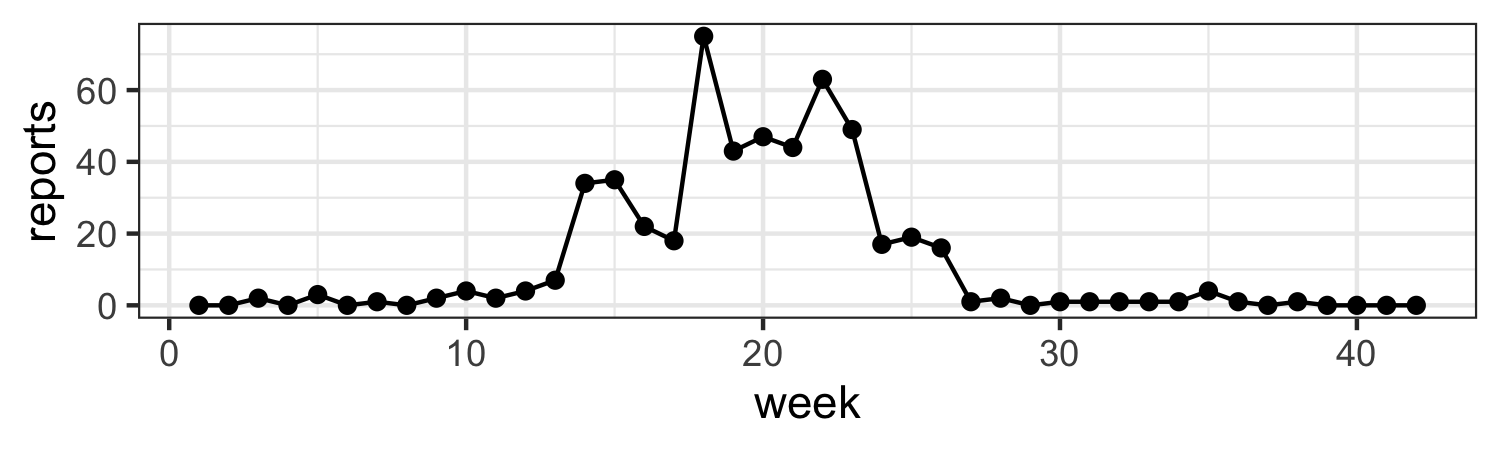
\includegraphics{tmp//figure/meas-data2-1.png}
\end{center}
\end{frame}

\begin{frame}[fragile,allowframebreaks]{The SIR as a POMP model for
measles}
\phantomsection\label{the-sir-as-a-pomp-model-for-measles}
Recall the simple SIR model and frame it as s POMP model:

\begin{center}
    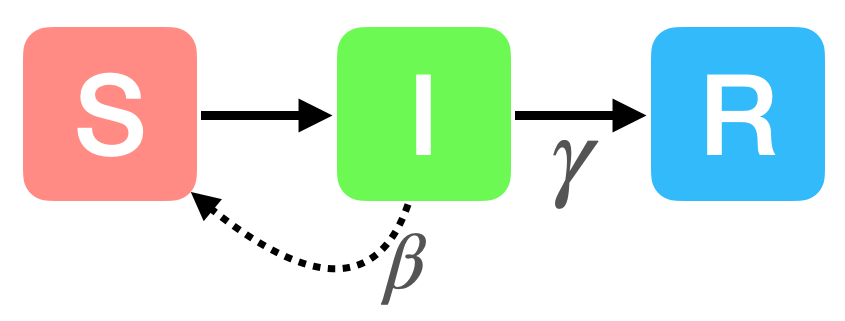
\includegraphics[height=2cm]{../graphics/simple-sir.png}
\end{center}

\begin{itemize}
\item
  The \textbf{unobserved states}: \(S(t)\), \(I(t)\), \(R(t)\), the
  numbers of individuals in the S, I, and R compartments, respectively.
\item
  The constant population size: \(N=S(t)+I(t)+R(t)\), as fixed at the
  known population size of 38,000.
\item
  \textbf{Flows} move from one compartment to another over any
  particular time interval are modeled as \emph{stochastic processes}.
\item
  \textbf{Demographic stochasticity}: each individual in a compartment
  at any given time faces the same risk of exiting the compartment; the
  unavoidable randomness that arises from chance events occurring in a
  discrete and finite population.
\end{itemize}

\framebreak

Recall the application of the Euler's method to a stochastic SIR model.

\begin{itemize}
\tightlist
\item
  \(\Delta N_{SI}\) and \(\Delta N_{IR}\): the flows from S to I and
  from I to R over interval \(\Delta t\), respectively:
\end{itemize}

\[
\begin{aligned}
    \Delta N_{SI} &\sim \mathrm{Binomial}\left(S, 1-e^{-\beta\frac{I}{N}\Delta t}\right),\\
    \Delta N_{IR} &\sim \mathrm{Binomial}\left(I, 1-e^{-\gamma\Delta t}\right).
\end{aligned}
\]

\framebreak

\begin{itemize}
\tightlist
\item
  Implement the dynamics in \texttt{pomp} as an R function:
\end{itemize}

\begin{Shaded}
\begin{Highlighting}[]
\NormalTok{sir\_stoch }\OtherTok{\textless{}{-}} \ControlFlowTok{function}\NormalTok{ (S, I, R, N, Beta, Gamma, delta.t, ...) \{}
\NormalTok{  dN\_SI }\OtherTok{\textless{}{-}} \FunctionTok{rbinom}\NormalTok{(}\AttributeTok{n=}\DecValTok{1}\NormalTok{,}\AttributeTok{size=}\NormalTok{S,}\AttributeTok{prob=}\DecValTok{1}\SpecialCharTok{{-}}\FunctionTok{exp}\NormalTok{(}\SpecialCharTok{{-}}\NormalTok{Beta}\SpecialCharTok{*}\NormalTok{I}\SpecialCharTok{/}\NormalTok{N}\SpecialCharTok{*}\NormalTok{delta.t))}
\NormalTok{  dN\_IR }\OtherTok{\textless{}{-}} \FunctionTok{rbinom}\NormalTok{(}\AttributeTok{n=}\DecValTok{1}\NormalTok{,}\AttributeTok{size=}\NormalTok{I,}\AttributeTok{prob=}\DecValTok{1}\SpecialCharTok{{-}}\FunctionTok{exp}\NormalTok{(}\SpecialCharTok{{-}}\NormalTok{Gamma}\SpecialCharTok{*}\NormalTok{delta.t))}
\NormalTok{  S }\OtherTok{\textless{}{-}}\NormalTok{ S }\SpecialCharTok{{-}}\NormalTok{ dN\_SI}
\NormalTok{  I }\OtherTok{\textless{}{-}}\NormalTok{ I }\SpecialCharTok{+}\NormalTok{ dN\_SI }\SpecialCharTok{{-}}\NormalTok{ dN\_IR}
\NormalTok{  R }\OtherTok{\textless{}{-}}\NormalTok{ R }\SpecialCharTok{+}\NormalTok{ dN\_IR}
  \FunctionTok{c}\NormalTok{(}\AttributeTok{S =}\NormalTok{ S, }\AttributeTok{I =}\NormalTok{ I, }\AttributeTok{R =}\NormalTok{ R)}
\NormalTok{\}}
\end{Highlighting}
\end{Shaded}

\begin{itemize}
\tightlist
\item
  Note that, for a deterministic SIR model:
\end{itemize}

\begin{Shaded}
\begin{Highlighting}[]
\NormalTok{dN\_SI }\OtherTok{\textless{}{-}}\NormalTok{ Beta}\SpecialCharTok{*}\NormalTok{S}\SpecialCharTok{*}\NormalTok{I}\SpecialCharTok{/}\NormalTok{N}\SpecialCharTok{*}\NormalTok{delta.t}
\NormalTok{dN\_IR }\OtherTok{\textless{}{-}}\NormalTok{ Gamma}\SpecialCharTok{*}\NormalTok{I}\SpecialCharTok{*}\NormalTok{delta.t}
\end{Highlighting}
\end{Shaded}

\framebreak

We can implement the initialization function with the following
assumptions:

\begin{itemize}
\item
  Assume the dynamics starts at week 0, \(t0=0\).
\item
  At \(t0\), assume the initial number of infection is 1, that is
  \(I=1\).
\item
  The initial number of susceptible is unknown, so we'll treat this
  fraction, \(\eta\), as a parameter to be estimated.
\end{itemize}

\begin{Shaded}
\begin{Highlighting}[]
\NormalTok{sir\_rinit }\OtherTok{\textless{}{-}} \ControlFlowTok{function}\NormalTok{ (N, Eta, ...) \{}
  \FunctionTok{c}\NormalTok{(}\AttributeTok{S =} \FunctionTok{round}\NormalTok{(N}\SpecialCharTok{*}\NormalTok{Eta), }\AttributeTok{I =} \DecValTok{1}\NormalTok{, }\AttributeTok{R =} \FunctionTok{round}\NormalTok{(N}\SpecialCharTok{*}\NormalTok{(}\DecValTok{1}\SpecialCharTok{{-}}\NormalTok{Eta)))}
\NormalTok{\}}
\end{Highlighting}
\end{Shaded}

\framebreak

With the initialization function \texttt{sir\_rinit} and the process
function \texttt{sir\_stoch}, we can build a \texttt{pomp} object with
these two components and the data:

\begin{Shaded}
\begin{Highlighting}[]
\FunctionTok{library}\NormalTok{(pomp)}
\NormalTok{meas }\SpecialCharTok{|\textgreater{}}
  \FunctionTok{pomp}\NormalTok{(}
    \AttributeTok{times=}\StringTok{"week"}\NormalTok{,}\AttributeTok{t0=}\DecValTok{0}\NormalTok{,}
    \AttributeTok{rprocess=}\FunctionTok{euler}\NormalTok{(sir\_stoch,}\AttributeTok{delta.t=}\DecValTok{1}\SpecialCharTok{/}\DecValTok{7}\NormalTok{),}
    \AttributeTok{rinit=}\NormalTok{sir\_rinit}
\NormalTok{  ) }\OtherTok{{-}\textgreater{}}\NormalTok{ measSIR}
\end{Highlighting}
\end{Shaded}

\begin{itemize}
\tightlist
\item
  Question: what do \texttt{times="week"} and \texttt{delta.t=1/7}
  indicate?
\end{itemize}

\framebreak

\begin{itemize}
\item
  Assume the \textbf{observations}, the \texttt{reports}, result from a
  process by which new infections are diagnosed in a hospital and
  reported with probability \(\rho\).
\item
  The diagnosed infections are immediately hospitalized, therefore, they
  have, presumably, a much lower transmission rate; let's assume each
  \emph{week's} reports as being related to the number of individuals
  who have moved from I to R over the course of that week.
\item
  We then define a new variable, \(H\), that tracks these daily counts.
\end{itemize}

\framebreak

We now can modify the R functions to incorporate the new variable \(H\):

\begin{Shaded}
\begin{Highlighting}[]
\NormalTok{sir\_stoch }\OtherTok{\textless{}{-}} \ControlFlowTok{function}\NormalTok{ (S, I, R, N, Beta, Gamma, delta.t, H, ...) \{}
\NormalTok{  dN\_SI }\OtherTok{\textless{}{-}} \FunctionTok{rbinom}\NormalTok{(}\AttributeTok{n=}\DecValTok{1}\NormalTok{,}\AttributeTok{size=}\NormalTok{S,}\AttributeTok{prob=}\DecValTok{1}\SpecialCharTok{{-}}\FunctionTok{exp}\NormalTok{(}\SpecialCharTok{{-}}\NormalTok{Beta}\SpecialCharTok{*}\NormalTok{I}\SpecialCharTok{/}\NormalTok{N}\SpecialCharTok{*}\NormalTok{delta.t))}
\NormalTok{  dN\_IR }\OtherTok{\textless{}{-}} \FunctionTok{rbinom}\NormalTok{(}\AttributeTok{n=}\DecValTok{1}\NormalTok{,}\AttributeTok{size=}\NormalTok{I,}\AttributeTok{prob=}\DecValTok{1}\SpecialCharTok{{-}}\FunctionTok{exp}\NormalTok{(}\SpecialCharTok{{-}}\NormalTok{Gamma}\SpecialCharTok{*}\NormalTok{delta.t))}
\NormalTok{  S }\OtherTok{\textless{}{-}}\NormalTok{ S }\SpecialCharTok{{-}}\NormalTok{ dN\_SI}
\NormalTok{  I }\OtherTok{\textless{}{-}}\NormalTok{ I }\SpecialCharTok{+}\NormalTok{ dN\_SI }\SpecialCharTok{{-}}\NormalTok{ dN\_IR}
\NormalTok{  R }\OtherTok{\textless{}{-}}\NormalTok{ R }\SpecialCharTok{+}\NormalTok{ dN\_IR}
\NormalTok{  H }\OtherTok{\textless{}{-}}\NormalTok{ H }\SpecialCharTok{+}\NormalTok{ dN\_IR}
  \FunctionTok{c}\NormalTok{(}\AttributeTok{S =}\NormalTok{ S, }\AttributeTok{I =}\NormalTok{ I, }\AttributeTok{R =}\NormalTok{ R, }\AttributeTok{H =}\NormalTok{ H)}
\NormalTok{\}}

\NormalTok{sir\_rinit }\OtherTok{\textless{}{-}} \ControlFlowTok{function}\NormalTok{ (N, Eta, ...) \{}
  \FunctionTok{c}\NormalTok{(}\AttributeTok{S =} \FunctionTok{round}\NormalTok{(N}\SpecialCharTok{*}\NormalTok{Eta), }\AttributeTok{I =} \DecValTok{1}\NormalTok{, }\AttributeTok{R =} \FunctionTok{round}\NormalTok{(N}\SpecialCharTok{*}\NormalTok{(}\DecValTok{1}\SpecialCharTok{{-}}\NormalTok{Eta)), }\AttributeTok{H =} \DecValTok{0}\NormalTok{)}
\NormalTok{\}}
\end{Highlighting}
\end{Shaded}

\framebreak

Note that, we are so far accounting for the \emph{flows} between
compartments by days, while the \texttt{reports} are weekly cases. Since
we want \(H\) to tally only the incidence over the week, we'll need to
reset it to zero at the beginning of each week. Thus, in \texttt{pomp}
terminology, \(H\) is an \textbf{accumulator variable}. We accomplish
this using the \texttt{accumvars} argument to \texttt{pomp} when build
the object:

\begin{Shaded}
\begin{Highlighting}[]
\NormalTok{measSIR }\SpecialCharTok{|\textgreater{}}
  \FunctionTok{pomp}\NormalTok{(}
    \AttributeTok{rprocess=}\FunctionTok{euler}\NormalTok{(sir\_stoch,}\AttributeTok{delta.t=}\DecValTok{1}\SpecialCharTok{/}\DecValTok{7}\NormalTok{),}
    \AttributeTok{rinit=}\NormalTok{sir\_rinit, }
    \AttributeTok{accumvars=}\StringTok{"H"}
\NormalTok{  ) }\OtherTok{{-}\textgreater{}}\NormalTok{ measSIR}
\end{Highlighting}
\end{Shaded}

\begin{itemize}
\tightlist
\item
  Question: what does that mean by running a \texttt{pomp} function with
  the \texttt{pomp} object \texttt{measSIR}?
\end{itemize}

\framebreak

Last but not least, we need to define a \textbf{measurement model} to
relate the \textbf{observations}, \texttt{reports}, to the
\textbf{unobserved} accumulative state, \(H\).

\begin{itemize}
\tightlist
\item
  We will model the data by a negative binomial variable,
  \[\mathrm{reports}_t \sim \dist{NegBin}{\rho\,H(t),k}.\] with mean
  \(\rho\,H(t)\) and variance \(\rho H(t)+ \big(\rho H(t)\big)^2/k\).
  The binomial distribution does not have a separate variance parameter.
\end{itemize}

\framebreak

\begin{itemize}
\tightlist
\item
  To include the observations in the model, we must write either a
  \texttt{dmeasure} or an \texttt{rmeasure} component, or both:
\end{itemize}

\begin{Shaded}
\begin{Highlighting}[]
\NormalTok{sir\_dmeas }\OtherTok{\textless{}{-}} \ControlFlowTok{function}\NormalTok{ (reports, H, Rho, k, log, ...) \{}
  \FunctionTok{dnbinom}\NormalTok{(}\AttributeTok{x=}\NormalTok{reports, }\AttributeTok{size=}\NormalTok{k, }\AttributeTok{mu=}\NormalTok{Rho}\SpecialCharTok{*}\NormalTok{H, }\AttributeTok{log=}\NormalTok{log)}
\NormalTok{\}}

\NormalTok{sir\_rmeas }\OtherTok{\textless{}{-}} \ControlFlowTok{function}\NormalTok{ (H, Rho, k, ...) \{}
  \FunctionTok{c}\NormalTok{(}\AttributeTok{reports=}\FunctionTok{rnbinom}\NormalTok{(}\AttributeTok{n=}\DecValTok{1}\NormalTok{, }\AttributeTok{size=}\NormalTok{k, }\AttributeTok{mu=}\NormalTok{Rho}\SpecialCharTok{*}\NormalTok{H))}
\NormalTok{\}}
\end{Highlighting}
\end{Shaded}

\framebreak

Eventually, we can add these two components to the previous
\texttt{measSIR} object to update the \texttt{dmeasure} and
\texttt{rmeasure} arguments:

\begin{Shaded}
\begin{Highlighting}[]
\NormalTok{measSIR }\SpecialCharTok{|\textgreater{}}
  \FunctionTok{pomp}\NormalTok{(}
    \AttributeTok{rmeasure=}\NormalTok{sir\_rmeas,}
    \AttributeTok{dmeasure=}\NormalTok{sir\_dmeas}
\NormalTok{  ) }\OtherTok{{-}\textgreater{}}\NormalTok{ measSIR}
\end{Highlighting}
\end{Shaded}
\end{frame}

\section{C snippets}\label{c-snippets}

\begin{frame}[fragile]{Specifying model components using C snippets}
\phantomsection\label{specifying-model-components-using-c-snippets}
\begin{itemize}
\item
  Although we can always specify basic model components using \texttt{R}
  functions, as above, we`ll typically want the computational speed-up
  that we can obtain only by using compiled native code.
\item
  pomp provides a facility for doing so with ease, using \emph{C
  snippets}.
\item
  C snippets are small pieces of C code used to specify basic model
  components.
\end{itemize}
\end{frame}

\begin{frame}[fragile]
\begin{itemize}
\tightlist
\item
  For example, a C snippet encoding the rprocess for an \texttt{sir}
  model is as follows.
\end{itemize}

\begin{Shaded}
\begin{Highlighting}[]
\NormalTok{    sir\_step }\OtherTok{\textless{}{-}} \FunctionTok{Csnippet}\NormalTok{(}\StringTok{"}
\StringTok{      double dN\_SI = rbinom(S,1{-}exp({-}Beta*I/N*dt));}
\StringTok{      double dN\_IR = rbinom(I,1{-}exp({-}Gamma*dt));}
\StringTok{      S {-}= dN\_SI;}
\StringTok{      I += dN\_SI {-} dN\_IR;}
\StringTok{      R += dN\_IR;}
\StringTok{      H += dN\_IR;}
\StringTok{    "}\NormalTok{)}
\end{Highlighting}
\end{Shaded}

\textbf{Note:}

\begin{itemize}
\item
  It is necessary to define the data type for the real values
  \texttt{dN\_SI} and \texttt{dN\_IR} as \texttt{double}. The data type
  for states does not need to be defined at this stage and will be
  addressed later.
\item
  \texttt{rbinom} is a built-in function used to generate random values
  from a binomial distribution. For additional built-in distributions in
  R, you can refer to
  \href{https://github.com/atks/Rmath/blob/master/Rmath/Rmath.h}{this
  Rmath.h document}.
\item
  Remember to add a semicolon (\texttt{;}) after each line to ensure
  proper syntax.
\end{itemize}
\end{frame}

\begin{frame}[fragile]
\begin{itemize}
\tightlist
\item
  C snippets for the initializer and measurement model are:
\end{itemize}

\begin{Shaded}
\begin{Highlighting}[]
\NormalTok{    sir\_rinit }\OtherTok{\textless{}{-}} \FunctionTok{Csnippet}\NormalTok{(}\StringTok{"}
\StringTok{      S = nearbyint(Eta*N);}
\StringTok{      I = 1;}
\StringTok{      R = nearbyint((1{-}Eta)*N);}
\StringTok{      H = 0;}
\StringTok{    "}\NormalTok{)}
\NormalTok{    sir\_dmeas }\OtherTok{\textless{}{-}} \FunctionTok{Csnippet}\NormalTok{(}\StringTok{"}
\StringTok{      lik = dnbinom\_mu(reports,k,Rho*H,give\_log);}
\StringTok{    "}\NormalTok{)}
\NormalTok{    sir\_rmeas }\OtherTok{\textless{}{-}} \FunctionTok{Csnippet}\NormalTok{(}\StringTok{"}
\StringTok{      reports = rnbinom\_mu(k,Rho*H);}
\StringTok{    "}\NormalTok{)}
\end{Highlighting}
\end{Shaded}

\begin{itemize}
\item
  No need to define the type for likelihood \texttt{(lik)} here, as it
  is already predefined.
\item
  \texttt{nearbyint} is a built-in function used to find the closest
  integer to a given value.
\item
  \texttt{reports} is the variable name specified in your dataset.
\end{itemize}
\end{frame}

\begin{frame}[fragile]
\begin{itemize}
\tightlist
\item
  A call to \texttt{pomp} replaces the basic model components with
  these, much faster, implementations:
\end{itemize}

\begin{Shaded}
\begin{Highlighting}[]
\NormalTok{    measSIR }\SpecialCharTok{|\textgreater{}}
      \FunctionTok{pomp}\NormalTok{(}\AttributeTok{rprocess=}\FunctionTok{euler}\NormalTok{(sir\_step,}\AttributeTok{delta.t=}\DecValTok{1}\SpecialCharTok{/}\DecValTok{7}\NormalTok{),}
        \AttributeTok{rinit=}\NormalTok{sir\_rinit,}
        \AttributeTok{rmeasure=}\NormalTok{sir\_rmeas,}
        \AttributeTok{dmeasure=}\NormalTok{sir\_dmeas,}
        \AttributeTok{accumvars=}\StringTok{"H"}\NormalTok{,}
        \AttributeTok{statenames=}\FunctionTok{c}\NormalTok{(}\StringTok{"S"}\NormalTok{,}\StringTok{"I"}\NormalTok{,}\StringTok{"R"}\NormalTok{,}\StringTok{"H"}\NormalTok{),}
        \AttributeTok{paramnames=}\FunctionTok{c}\NormalTok{(}\StringTok{"Beta"}\NormalTok{,}\StringTok{"Gamma"}\NormalTok{,}\StringTok{"N"}\NormalTok{,}\StringTok{"Eta"}\NormalTok{,}\StringTok{"Rho"}\NormalTok{,}\StringTok{"k"}\NormalTok{)}
\NormalTok{      ) }\OtherTok{{-}\textgreater{}}\NormalTok{ measSIR\_C}
\end{Highlighting}
\end{Shaded}

\begin{itemize}
\tightlist
\item
  Note that, when using C snippets, one has to tell pomp which of the
  variables referenced in the C snippets are state variables and which
  are parameters. This is accomplished using the \texttt{statenames} and
  \texttt{paramnames} arguments.
\end{itemize}
\end{frame}

\begin{frame}[fragile,allowframebreaks]{Compare the running time between
R and CSnippet}
\phantomsection\label{compare-the-running-time-between-r-and-csnippet}
\begin{Shaded}
\begin{Highlighting}[]
\NormalTok{fR }\OtherTok{\textless{}{-}} \ControlFlowTok{function}\NormalTok{() \{measSIR }\SpecialCharTok{|\textgreater{}}
      \FunctionTok{simulate}\NormalTok{(}
        \AttributeTok{params=}\FunctionTok{c}\NormalTok{(}\AttributeTok{Beta=}\FloatTok{7.5}\NormalTok{,}\AttributeTok{Gamma=}\FloatTok{0.5}\NormalTok{,}\AttributeTok{Rho=}\FloatTok{0.5}\NormalTok{,}\AttributeTok{k=}\DecValTok{10}\NormalTok{,}
          \AttributeTok{Eta=}\FloatTok{0.03}\NormalTok{,}\AttributeTok{N=}\DecValTok{38000}\NormalTok{),}
        \AttributeTok{nsim=}\DecValTok{100}\NormalTok{,}\AttributeTok{format=}\StringTok{"data.frame"}\NormalTok{,}\AttributeTok{include.data=}\ConstantTok{TRUE}
\NormalTok{      )\} }
\NormalTok{fC }\OtherTok{\textless{}{-}} \ControlFlowTok{function}\NormalTok{() \{measSIR\_C }\SpecialCharTok{|\textgreater{}}
      \FunctionTok{simulate}\NormalTok{(}
        \AttributeTok{params=}\FunctionTok{c}\NormalTok{(}\AttributeTok{Beta=}\FloatTok{7.5}\NormalTok{,}\AttributeTok{Gamma=}\FloatTok{0.5}\NormalTok{,}\AttributeTok{Rho=}\FloatTok{0.5}\NormalTok{,}\AttributeTok{k=}\DecValTok{10}\NormalTok{,}
          \AttributeTok{Eta=}\FloatTok{0.03}\NormalTok{,}\AttributeTok{N=}\DecValTok{38000}\NormalTok{),}
        \AttributeTok{nsim=}\DecValTok{100}\NormalTok{,}\AttributeTok{format=}\StringTok{"data.frame"}\NormalTok{,}\AttributeTok{include.data=}\ConstantTok{TRUE}
\NormalTok{      )\} }
\NormalTok{res }\OtherTok{\textless{}{-}} \FunctionTok{microbenchmark}\NormalTok{(}\FunctionTok{fR}\NormalTok{(), }\FunctionTok{fC}\NormalTok{(), }\AttributeTok{times=}\DecValTok{100}\NormalTok{L)}
\end{Highlighting}
\end{Shaded}

\begin{center}
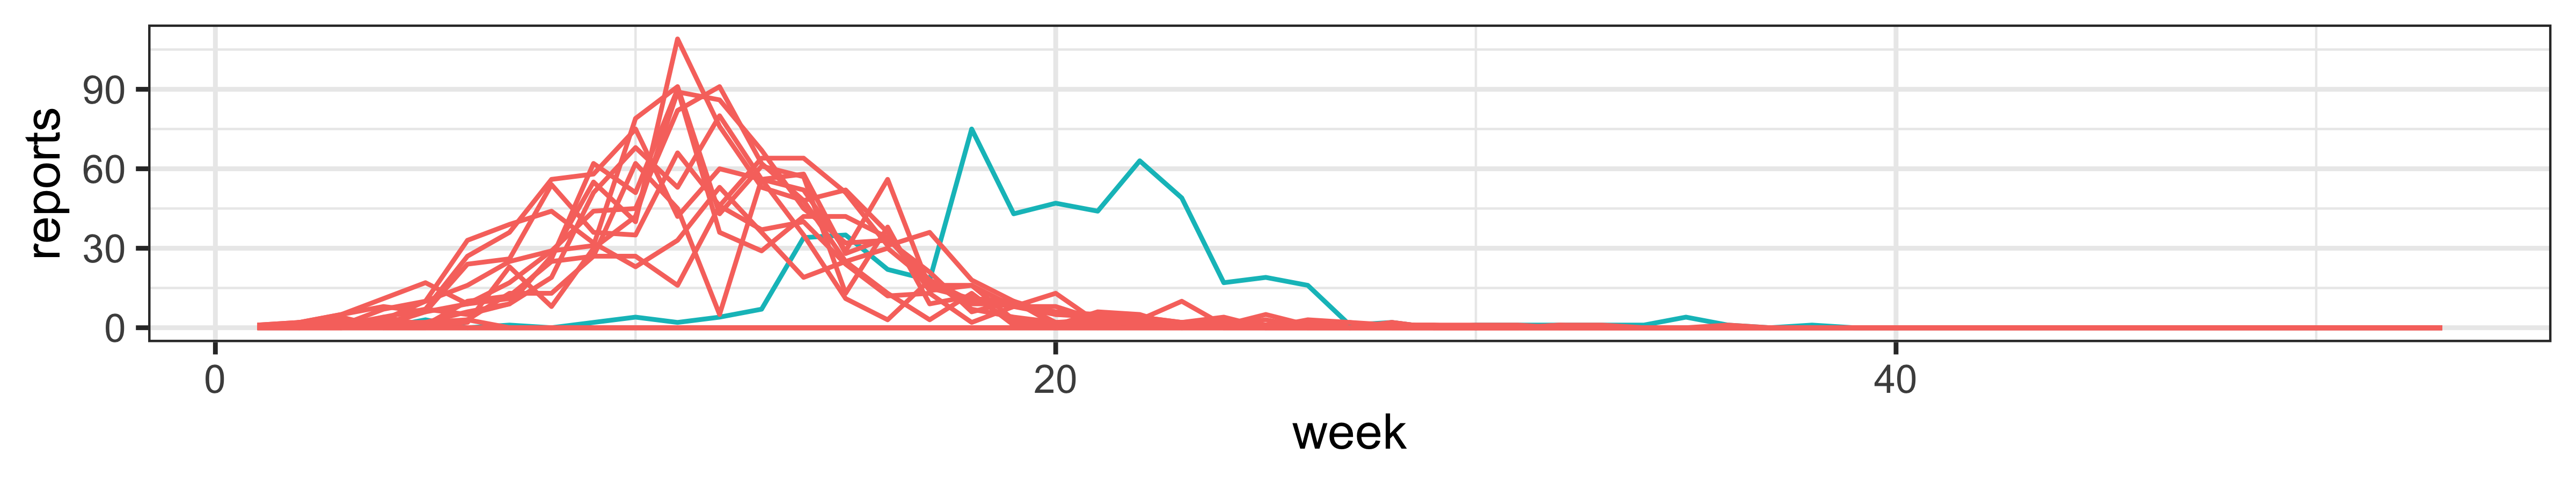
\includegraphics{tmp//figure/unnamed-chunk-2-1.png}
\end{center}

\begin{itemize}
\tightlist
\item
  We can tell from the summary table that CSnippet is approximate 50
  times faster than R.
\end{itemize}
\end{frame}

\section{Choosing parameters}\label{choosing-parameters}

\begin{frame}[fragile,allowframebreaks]{Guessing plausible parameter
values}
\phantomsection\label{guessing-plausible-parameter-values}
\begin{itemize}
\item
  To check the code is working properly, we simulate. This requires us
  to assign parameters. A little thought will get us some ballpark
  estimates.
\item
  Recall that \(\Rzero\) is the expected number of secondary infections
  resulting from one primary infection introduced into a fully
  susceptible population. For an SIR infection, one has that
  \(\Rzero\approx\frac{L}{A}\), where \(L\) is the lifespan of a host
  and \(A\) is the mean age of infection. Analysis of age-stratified
  serology data establish that the mean age of infection for measles
  during this period was around 4--5yr (Anderson and May 1991). Assuming
  a lifespan of 60--70yr, we have \(\Rzero\approx 15\).
\item
  The basic theory of SIR epidemics gives the final-size equation,
  \[\Rzero = -\frac{\log{(1-f)}}{f},\] where \(f\) is the final size of
  the epidemic---the fraction of those susceptible at the beginning of
  the outbreak who ultimately become infected. For \(\Rzero>5\), this
  equation predicts that \(f>0.99\).
\item
  In the data, it looks like there were a total of \(521\) infections.
  Assuming 50\% reporting, we have that \(S_0\approx1042\), so that
  \(\eta=\frac{S_0}{N}\approx`r mysignif(2*sum(meas\)reports)/38000,2)\textbackslash\$.
\item
  If the infectious period is roughly 2 weeks, then
  \(1/\mu_{IR} \approx 2~\text{wk}\) and
  \(\beta = \mu_{IR}\,\Rzero \approx 7.5~\text{wk}^{-1}\).
\item
  Let's simulate the model at these parameters.
\end{itemize}

\begin{Shaded}
\begin{Highlighting}[]
\NormalTok{    measSIR }\SpecialCharTok{|\textgreater{}}
      \FunctionTok{simulate}\NormalTok{(}
        \AttributeTok{params=}\FunctionTok{c}\NormalTok{(}\AttributeTok{Beta=}\FloatTok{7.5}\NormalTok{,}\AttributeTok{Gamma=}\FloatTok{0.5}\NormalTok{,}\AttributeTok{Rho=}\FloatTok{0.5}\NormalTok{,}\AttributeTok{k=}\DecValTok{10}\NormalTok{, }\AttributeTok{Eta=}\FloatTok{0.03}\NormalTok{,}\AttributeTok{N=}\DecValTok{38000}\NormalTok{),}
        \AttributeTok{nsim=}\DecValTok{20}\NormalTok{,}\AttributeTok{format=}\StringTok{"data.frame"}\NormalTok{,}\AttributeTok{include.data=}\ConstantTok{TRUE}
\NormalTok{      ) }\OtherTok{{-}\textgreater{}}\NormalTok{ sims}

\NormalTok{    sims }\SpecialCharTok{|\textgreater{}}
      \FunctionTok{ggplot}\NormalTok{(}\FunctionTok{aes}\NormalTok{(}\AttributeTok{x=}\NormalTok{week,}\AttributeTok{y=}\NormalTok{reports,}\AttributeTok{group=}\NormalTok{.id,}\AttributeTok{color=}\NormalTok{.id}\SpecialCharTok{==}\StringTok{"data"}\NormalTok{))}\SpecialCharTok{+}
      \FunctionTok{geom\_line}\NormalTok{()}\SpecialCharTok{+}
      \FunctionTok{guides}\NormalTok{(}\AttributeTok{color=}\StringTok{"none"}\NormalTok{)}
\end{Highlighting}
\end{Shaded}

\begin{center}
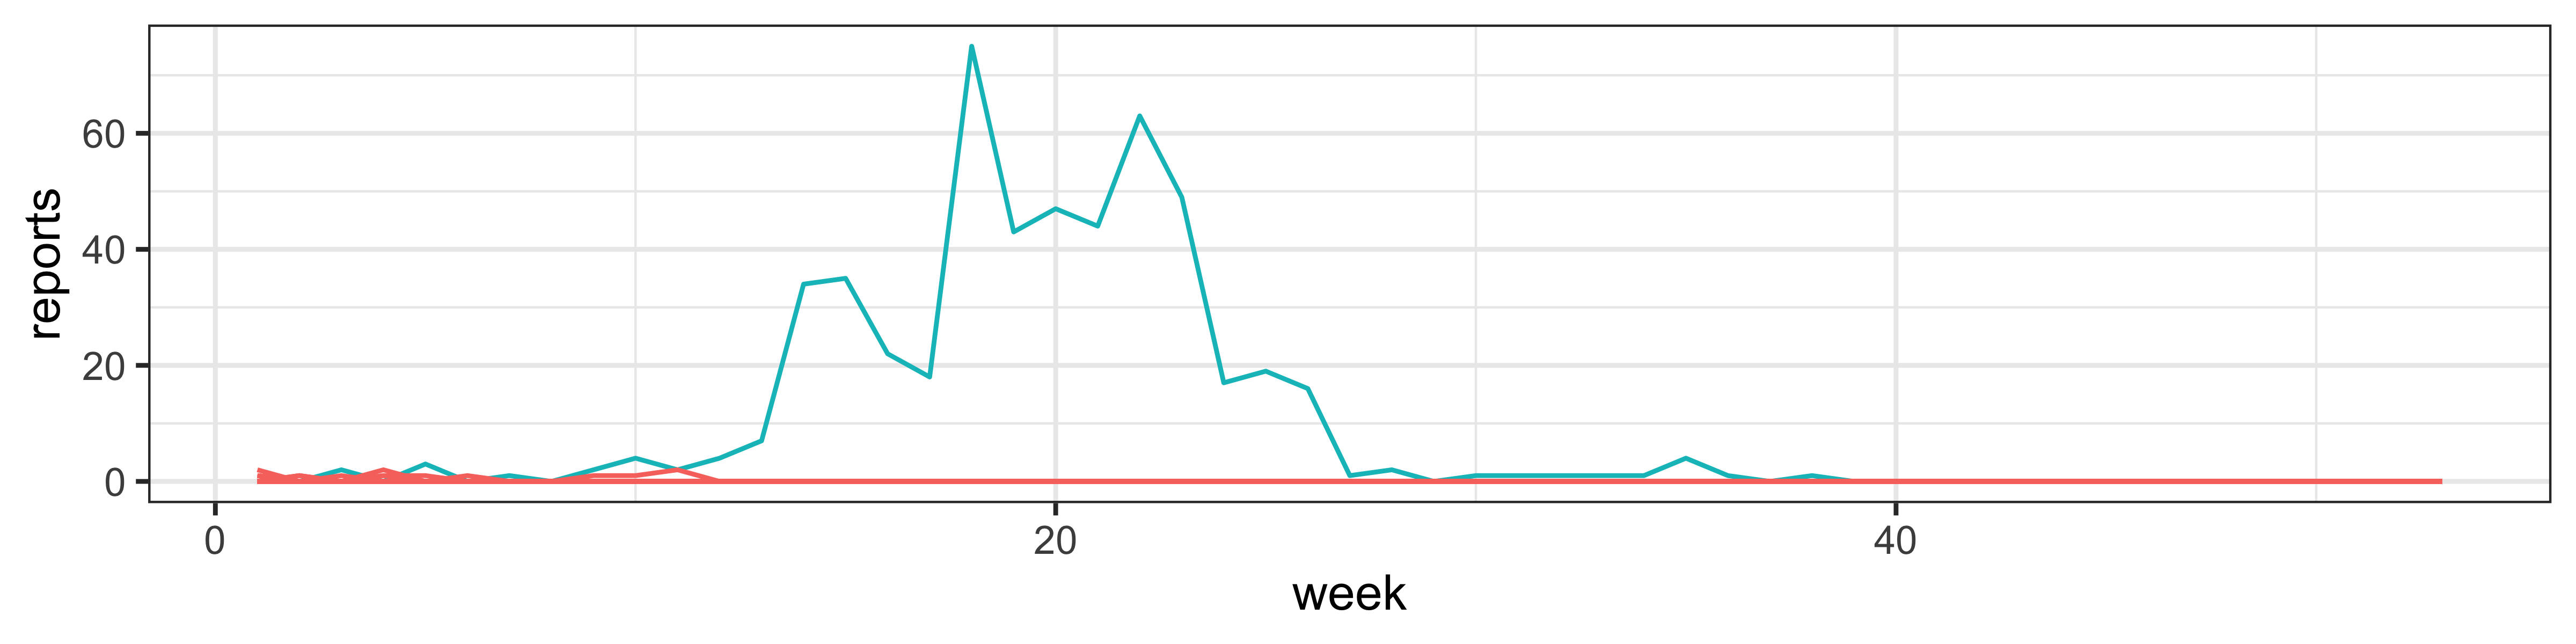
\includegraphics[width=8cm,height=\textheight]{tmp//figure/sir_sim1_plot-1.png}
\end{center}

The data are in blue; the 20 simulations are shown in red.

Clearly, this leaves something to be desired. In the exercises, you'll
see if this model can do better.
\end{frame}

\section{Exercises}\label{exercises}

\begin{frame}{Exercise: Explore the SIR model}
\phantomsection\label{exercise-explore-the-sir-model}
Fiddle with the parameters to see if you can't find a model for which
the data are a more plausible realization.
\end{frame}

\begin{frame}[fragile,allowframebreaks]{Worked solutions: Explore the
SIR model}
\phantomsection\label{worked-solutions-explore-the-sir-model}
In the simulated outbreaks, the overall incidence is much too low, and
the outbreak dies out after only a few weeks. To attempt to simulate
data for which the observed data is a more plausible realization, we
might try increasing the force of infection.

\begin{Shaded}
\begin{Highlighting}[]
\NormalTok{measSIR }\SpecialCharTok{|\textgreater{}}
  \FunctionTok{simulate}\NormalTok{(}\AttributeTok{params=}\FunctionTok{c}\NormalTok{(}\AttributeTok{Beta=}\DecValTok{25}\NormalTok{,}\AttributeTok{Gamma=}\FloatTok{0.5}\NormalTok{,}\AttributeTok{Rho=}\FloatTok{0.5}\NormalTok{,}\AttributeTok{k=}\DecValTok{10}\NormalTok{,}\AttributeTok{Eta=}\FloatTok{0.03}\NormalTok{,}\AttributeTok{N=}\DecValTok{38000}\NormalTok{),}
    \AttributeTok{nsim=}\DecValTok{20}\NormalTok{,}\AttributeTok{format=}\StringTok{"data.frame"}\NormalTok{,}\AttributeTok{include.data=}\ConstantTok{TRUE}\NormalTok{) }\SpecialCharTok{|\textgreater{}}
  \FunctionTok{ggplot}\NormalTok{(}\FunctionTok{aes}\NormalTok{(}\AttributeTok{x=}\NormalTok{week,}\AttributeTok{y=}\NormalTok{reports,}\AttributeTok{group=}\NormalTok{.id,}\AttributeTok{color=}\NormalTok{.id}\SpecialCharTok{==}\StringTok{"data"}\NormalTok{))}\SpecialCharTok{+}
  \FunctionTok{geom\_line}\NormalTok{()}\SpecialCharTok{+}
  \FunctionTok{guides}\NormalTok{(}\AttributeTok{color=}\StringTok{"none"}\NormalTok{)}
\end{Highlighting}
\end{Shaded}

\begin{center}
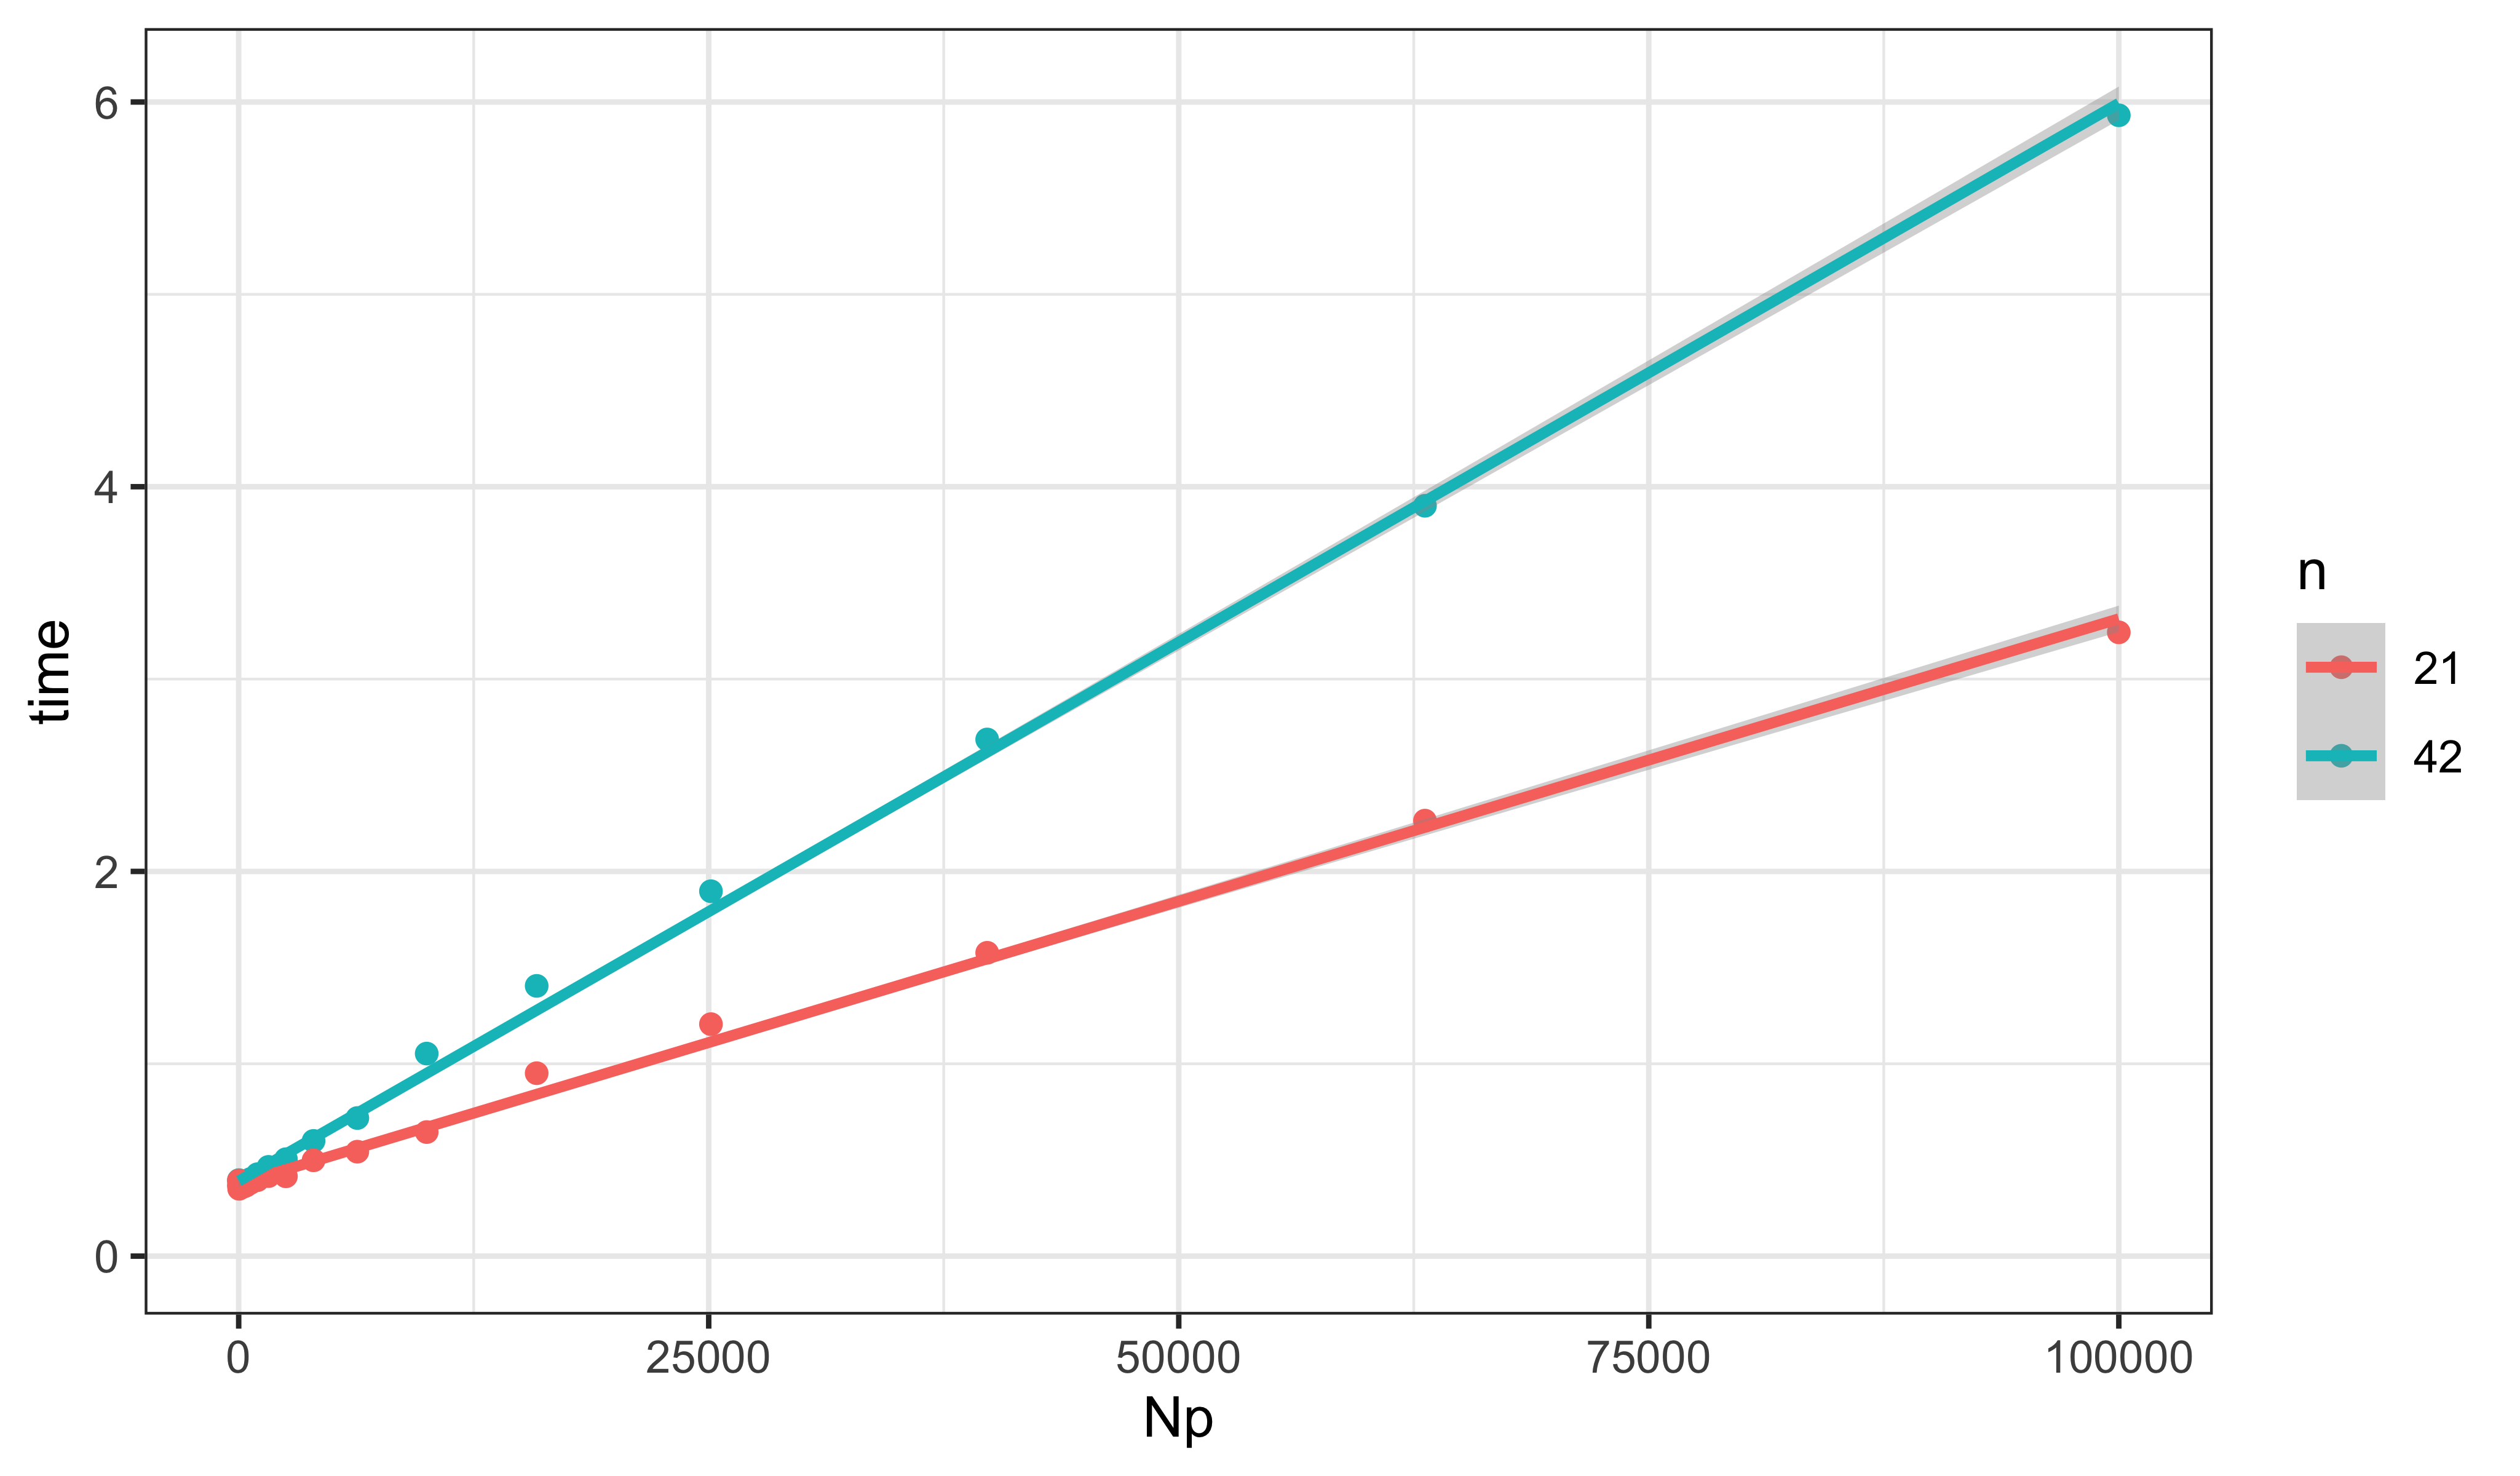
\includegraphics{tmp//figure/unnamed-chunk-3-1.png}
\end{center}
\end{frame}

\begin{frame}[fragile]
Taking it farther\ldots.

\begin{Shaded}
\begin{Highlighting}[]
\NormalTok{measSIR }\SpecialCharTok{|\textgreater{}}
  \FunctionTok{simulate}\NormalTok{(}\AttributeTok{params=}\FunctionTok{c}\NormalTok{(}\AttributeTok{Beta=}\DecValTok{40}\NormalTok{,}\AttributeTok{Gamma=}\FloatTok{0.5}\NormalTok{,}\AttributeTok{Rho=}\FloatTok{0.5}\NormalTok{,}\AttributeTok{k=}\DecValTok{10}\NormalTok{,}\AttributeTok{Eta=}\FloatTok{0.03}\NormalTok{,}\AttributeTok{N=}\DecValTok{38000}\NormalTok{),}
    \AttributeTok{nsim=}\DecValTok{20}\NormalTok{,}\AttributeTok{format=}\StringTok{"data.frame"}\NormalTok{,}\AttributeTok{include.data=}\ConstantTok{TRUE}\NormalTok{) }\SpecialCharTok{|\textgreater{}}
  \FunctionTok{ggplot}\NormalTok{(}\FunctionTok{aes}\NormalTok{(}\AttributeTok{x=}\NormalTok{week,}\AttributeTok{y=}\NormalTok{reports,}\AttributeTok{group=}\NormalTok{.id,}\AttributeTok{color=}\NormalTok{.id}\SpecialCharTok{==}\StringTok{"data"}\NormalTok{))}\SpecialCharTok{+}
  \FunctionTok{geom\_line}\NormalTok{()}\SpecialCharTok{+}
  \FunctionTok{guides}\NormalTok{(}\AttributeTok{color=}\StringTok{"none"}\NormalTok{)}
\end{Highlighting}
\end{Shaded}

\begin{center}
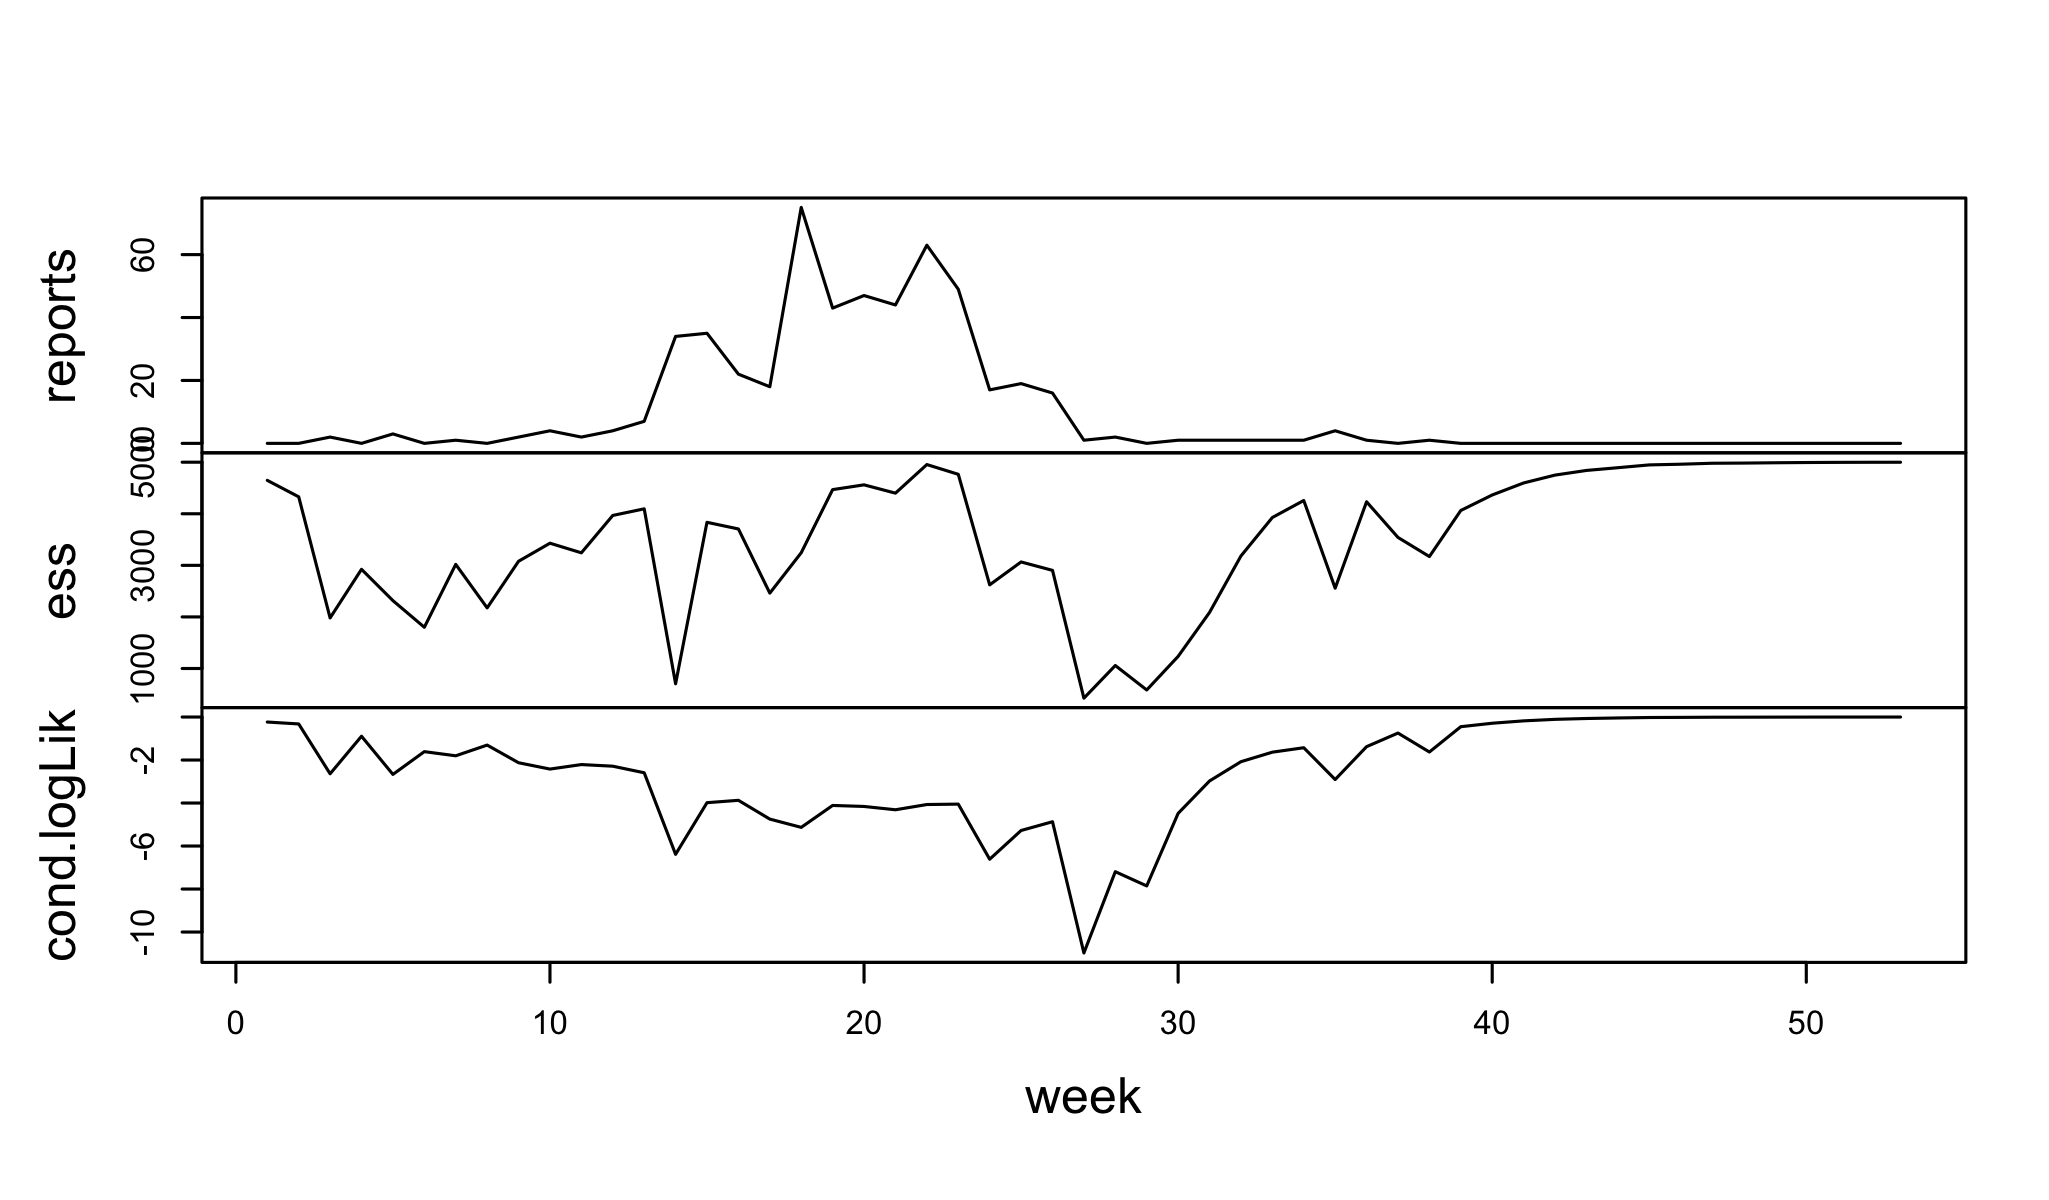
\includegraphics{tmp//figure/unnamed-chunk-4-1.png}
\end{center}
\end{frame}

\begin{frame}[fragile]
While this increases the overall incidence, the epidemic is now peaking
too quickly. To counteract this, we might try reducing the recovery
rate.

\begin{Shaded}
\begin{Highlighting}[]
\NormalTok{measSIR }\SpecialCharTok{|\textgreater{}}
  \FunctionTok{simulate}\NormalTok{(}\AttributeTok{params=}\FunctionTok{c}\NormalTok{(}\AttributeTok{Beta=}\DecValTok{40}\NormalTok{,}\AttributeTok{Gamma=}\FloatTok{0.2}\NormalTok{,}\AttributeTok{Rho=}\FloatTok{0.5}\NormalTok{,}\AttributeTok{k=}\DecValTok{10}\NormalTok{,}\AttributeTok{Eta=}\FloatTok{0.03}\NormalTok{,}\AttributeTok{N=}\DecValTok{38000}\NormalTok{),}
    \AttributeTok{nsim=}\DecValTok{20}\NormalTok{,}\AttributeTok{format=}\StringTok{"data.frame"}\NormalTok{,}\AttributeTok{include.data=}\ConstantTok{TRUE}\NormalTok{) }\SpecialCharTok{|\textgreater{}}
  \FunctionTok{ggplot}\NormalTok{(}\FunctionTok{aes}\NormalTok{(}\AttributeTok{x=}\NormalTok{week,}\AttributeTok{y=}\NormalTok{reports,}\AttributeTok{group=}\NormalTok{.id,}\AttributeTok{color=}\NormalTok{.id}\SpecialCharTok{==}\StringTok{"data"}\NormalTok{))}\SpecialCharTok{+}
  \FunctionTok{geom\_line}\NormalTok{()}\SpecialCharTok{+}
  \FunctionTok{guides}\NormalTok{(}\AttributeTok{color=}\StringTok{"none"}\NormalTok{)}
\end{Highlighting}
\end{Shaded}

\begin{center}
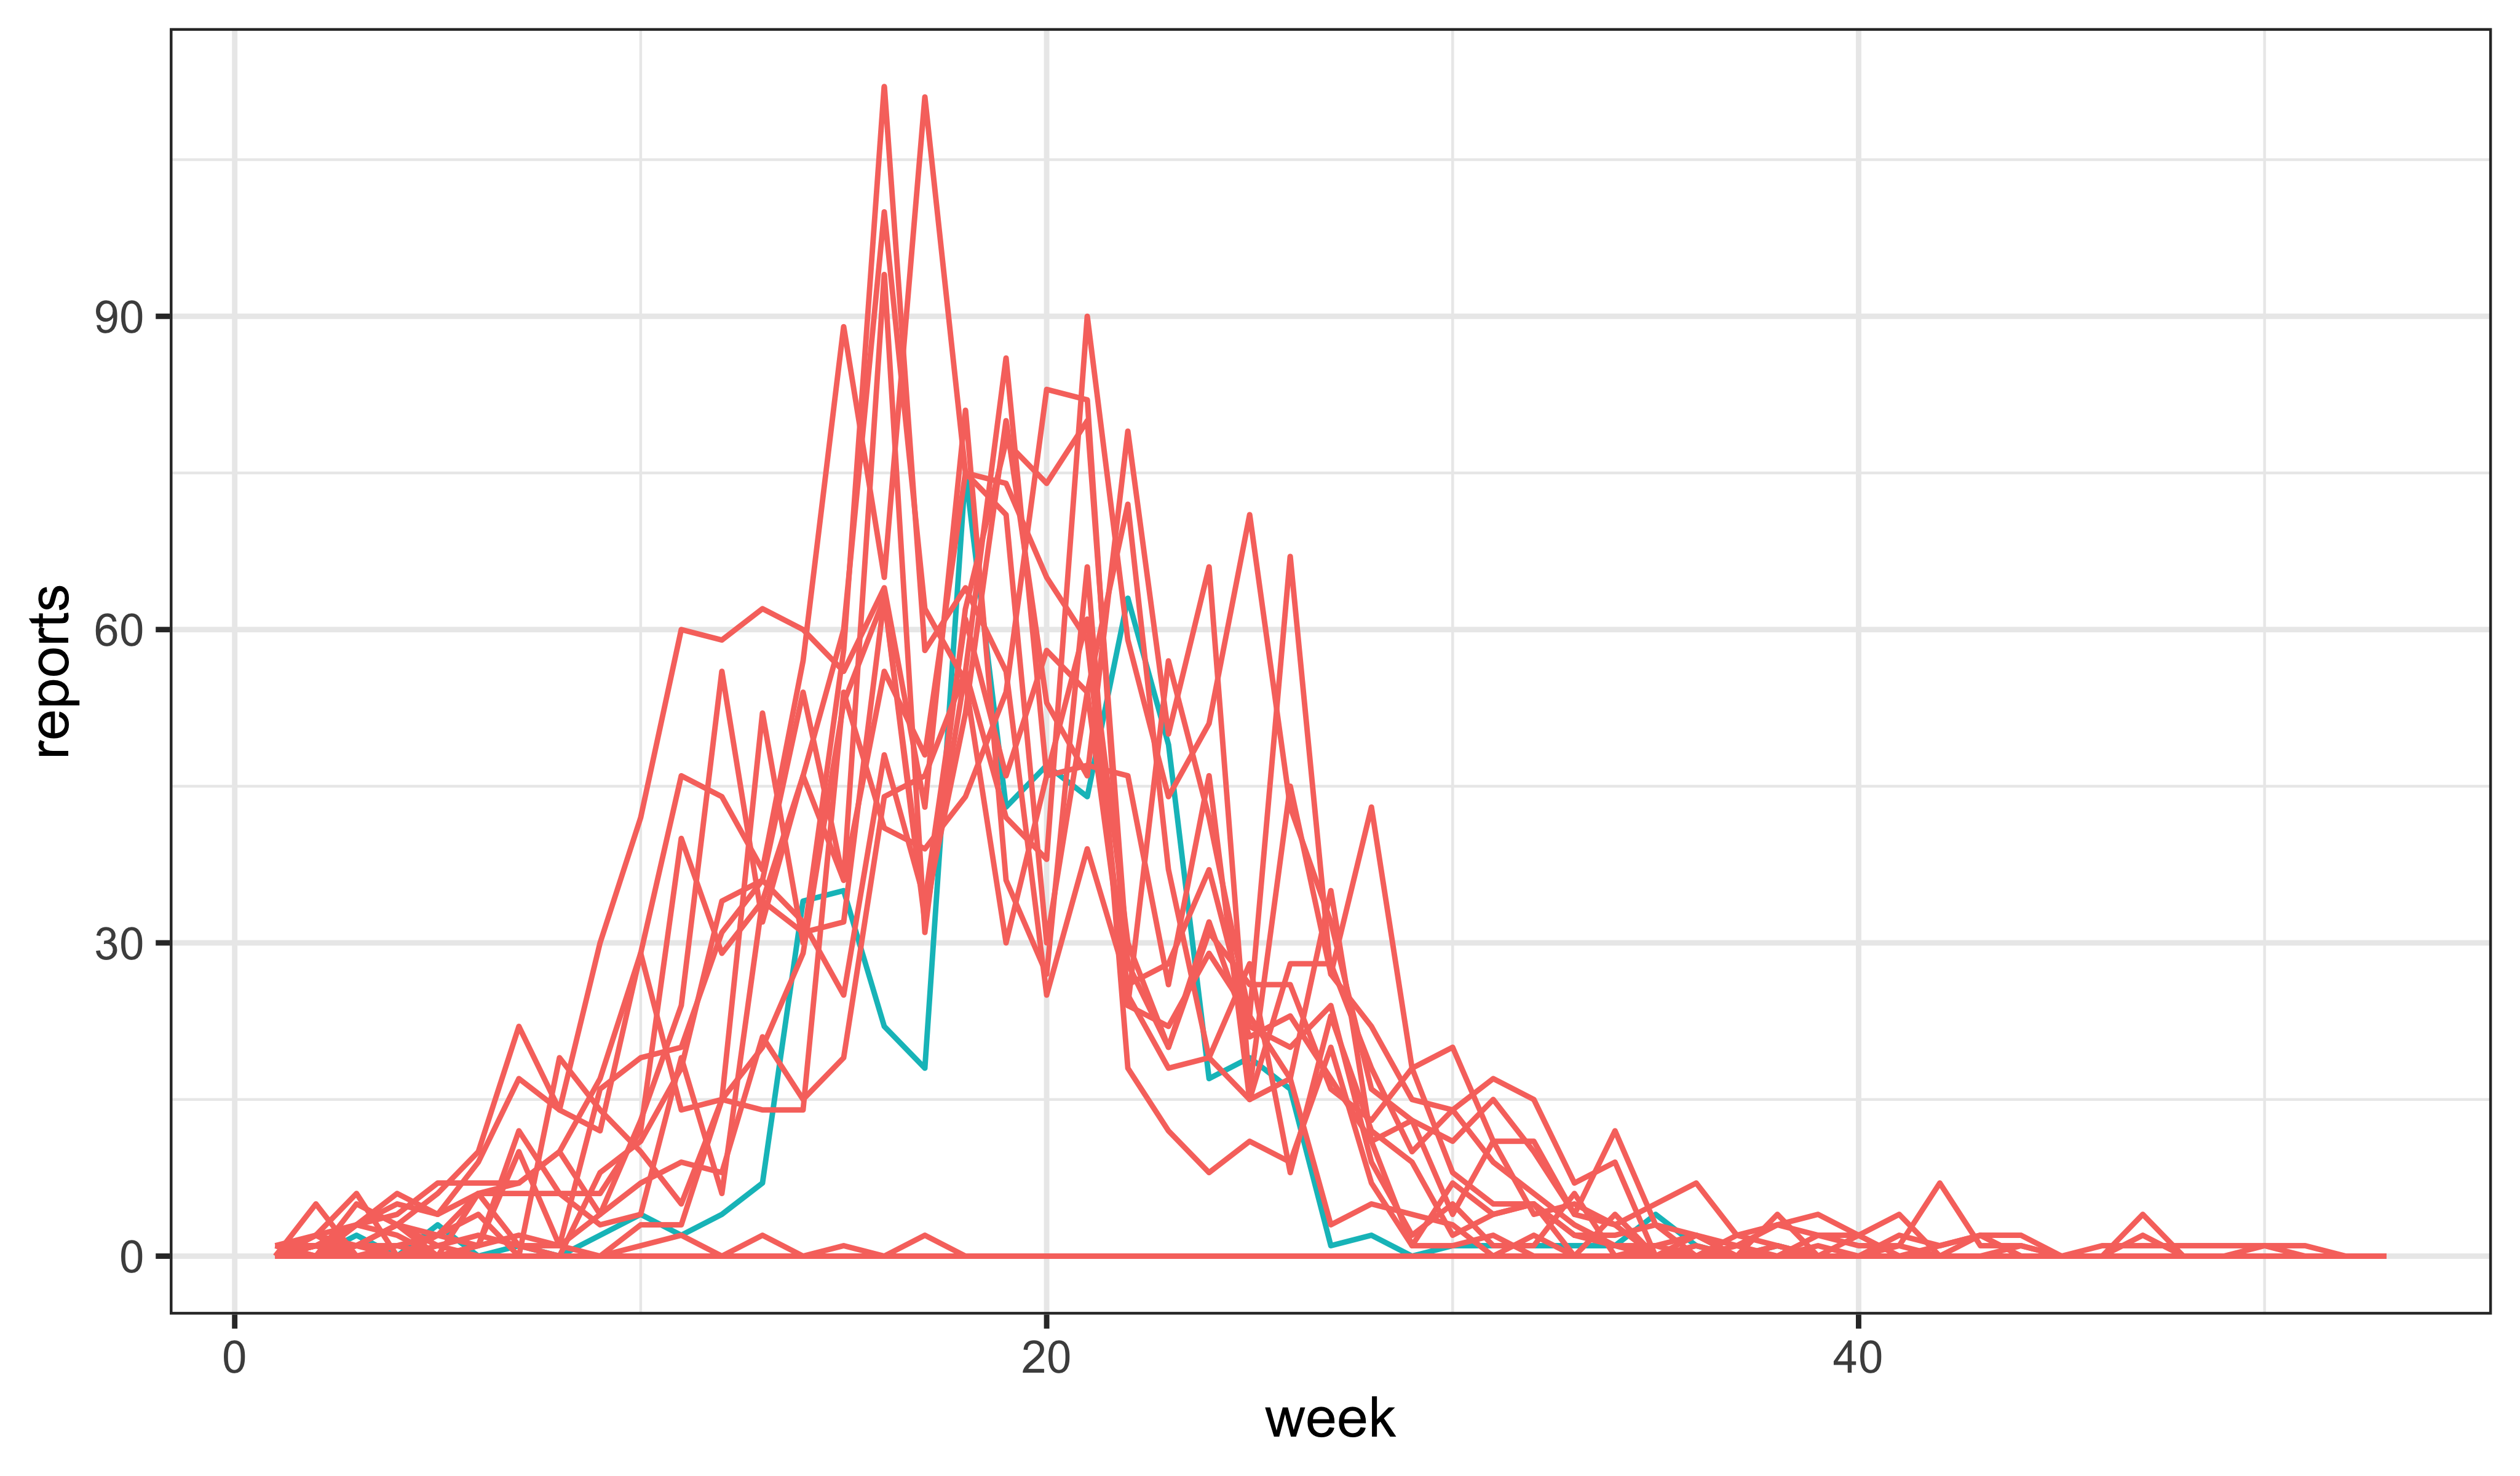
\includegraphics{tmp//figure/unnamed-chunk-5-1.png}
\end{center}
\end{frame}

\begin{frame}[fragile]
Additionally, we might have a look at the effects of changing the
initial susceptible fraction, \(\eta\). Indeed, it seems that it is
possible to get something not too awful to contemplate by just
manipulating \(\eta\):

\begin{Shaded}
\begin{Highlighting}[]
\NormalTok{measSIR }\SpecialCharTok{|\textgreater{}}
  \FunctionTok{simulate}\NormalTok{(}\AttributeTok{params=}\FunctionTok{c}\NormalTok{(}\AttributeTok{Beta=}\DecValTok{15}\NormalTok{,}\AttributeTok{Gamma=}\FloatTok{0.5}\NormalTok{,}\AttributeTok{Rho=}\FloatTok{0.5}\NormalTok{,}\AttributeTok{k=}\DecValTok{10}\NormalTok{,}\AttributeTok{Eta=}\FloatTok{0.06}\NormalTok{,}\AttributeTok{N=}\DecValTok{38000}\NormalTok{),}
    \AttributeTok{nsim=}\DecValTok{20}\NormalTok{,}\AttributeTok{format=}\StringTok{"data.frame"}\NormalTok{,}\AttributeTok{include.data=}\ConstantTok{TRUE}\NormalTok{) }\SpecialCharTok{|\textgreater{}}
  \FunctionTok{ggplot}\NormalTok{(}\FunctionTok{aes}\NormalTok{(}\AttributeTok{x=}\NormalTok{week,}\AttributeTok{y=}\NormalTok{reports,}\AttributeTok{group=}\NormalTok{.id,}\AttributeTok{color=}\NormalTok{.id}\SpecialCharTok{==}\StringTok{"data"}\NormalTok{))}\SpecialCharTok{+}
  \FunctionTok{geom\_line}\NormalTok{()}\SpecialCharTok{+}
  \FunctionTok{guides}\NormalTok{(}\AttributeTok{color=}\StringTok{"none"}\NormalTok{)}
\end{Highlighting}
\end{Shaded}

\begin{center}
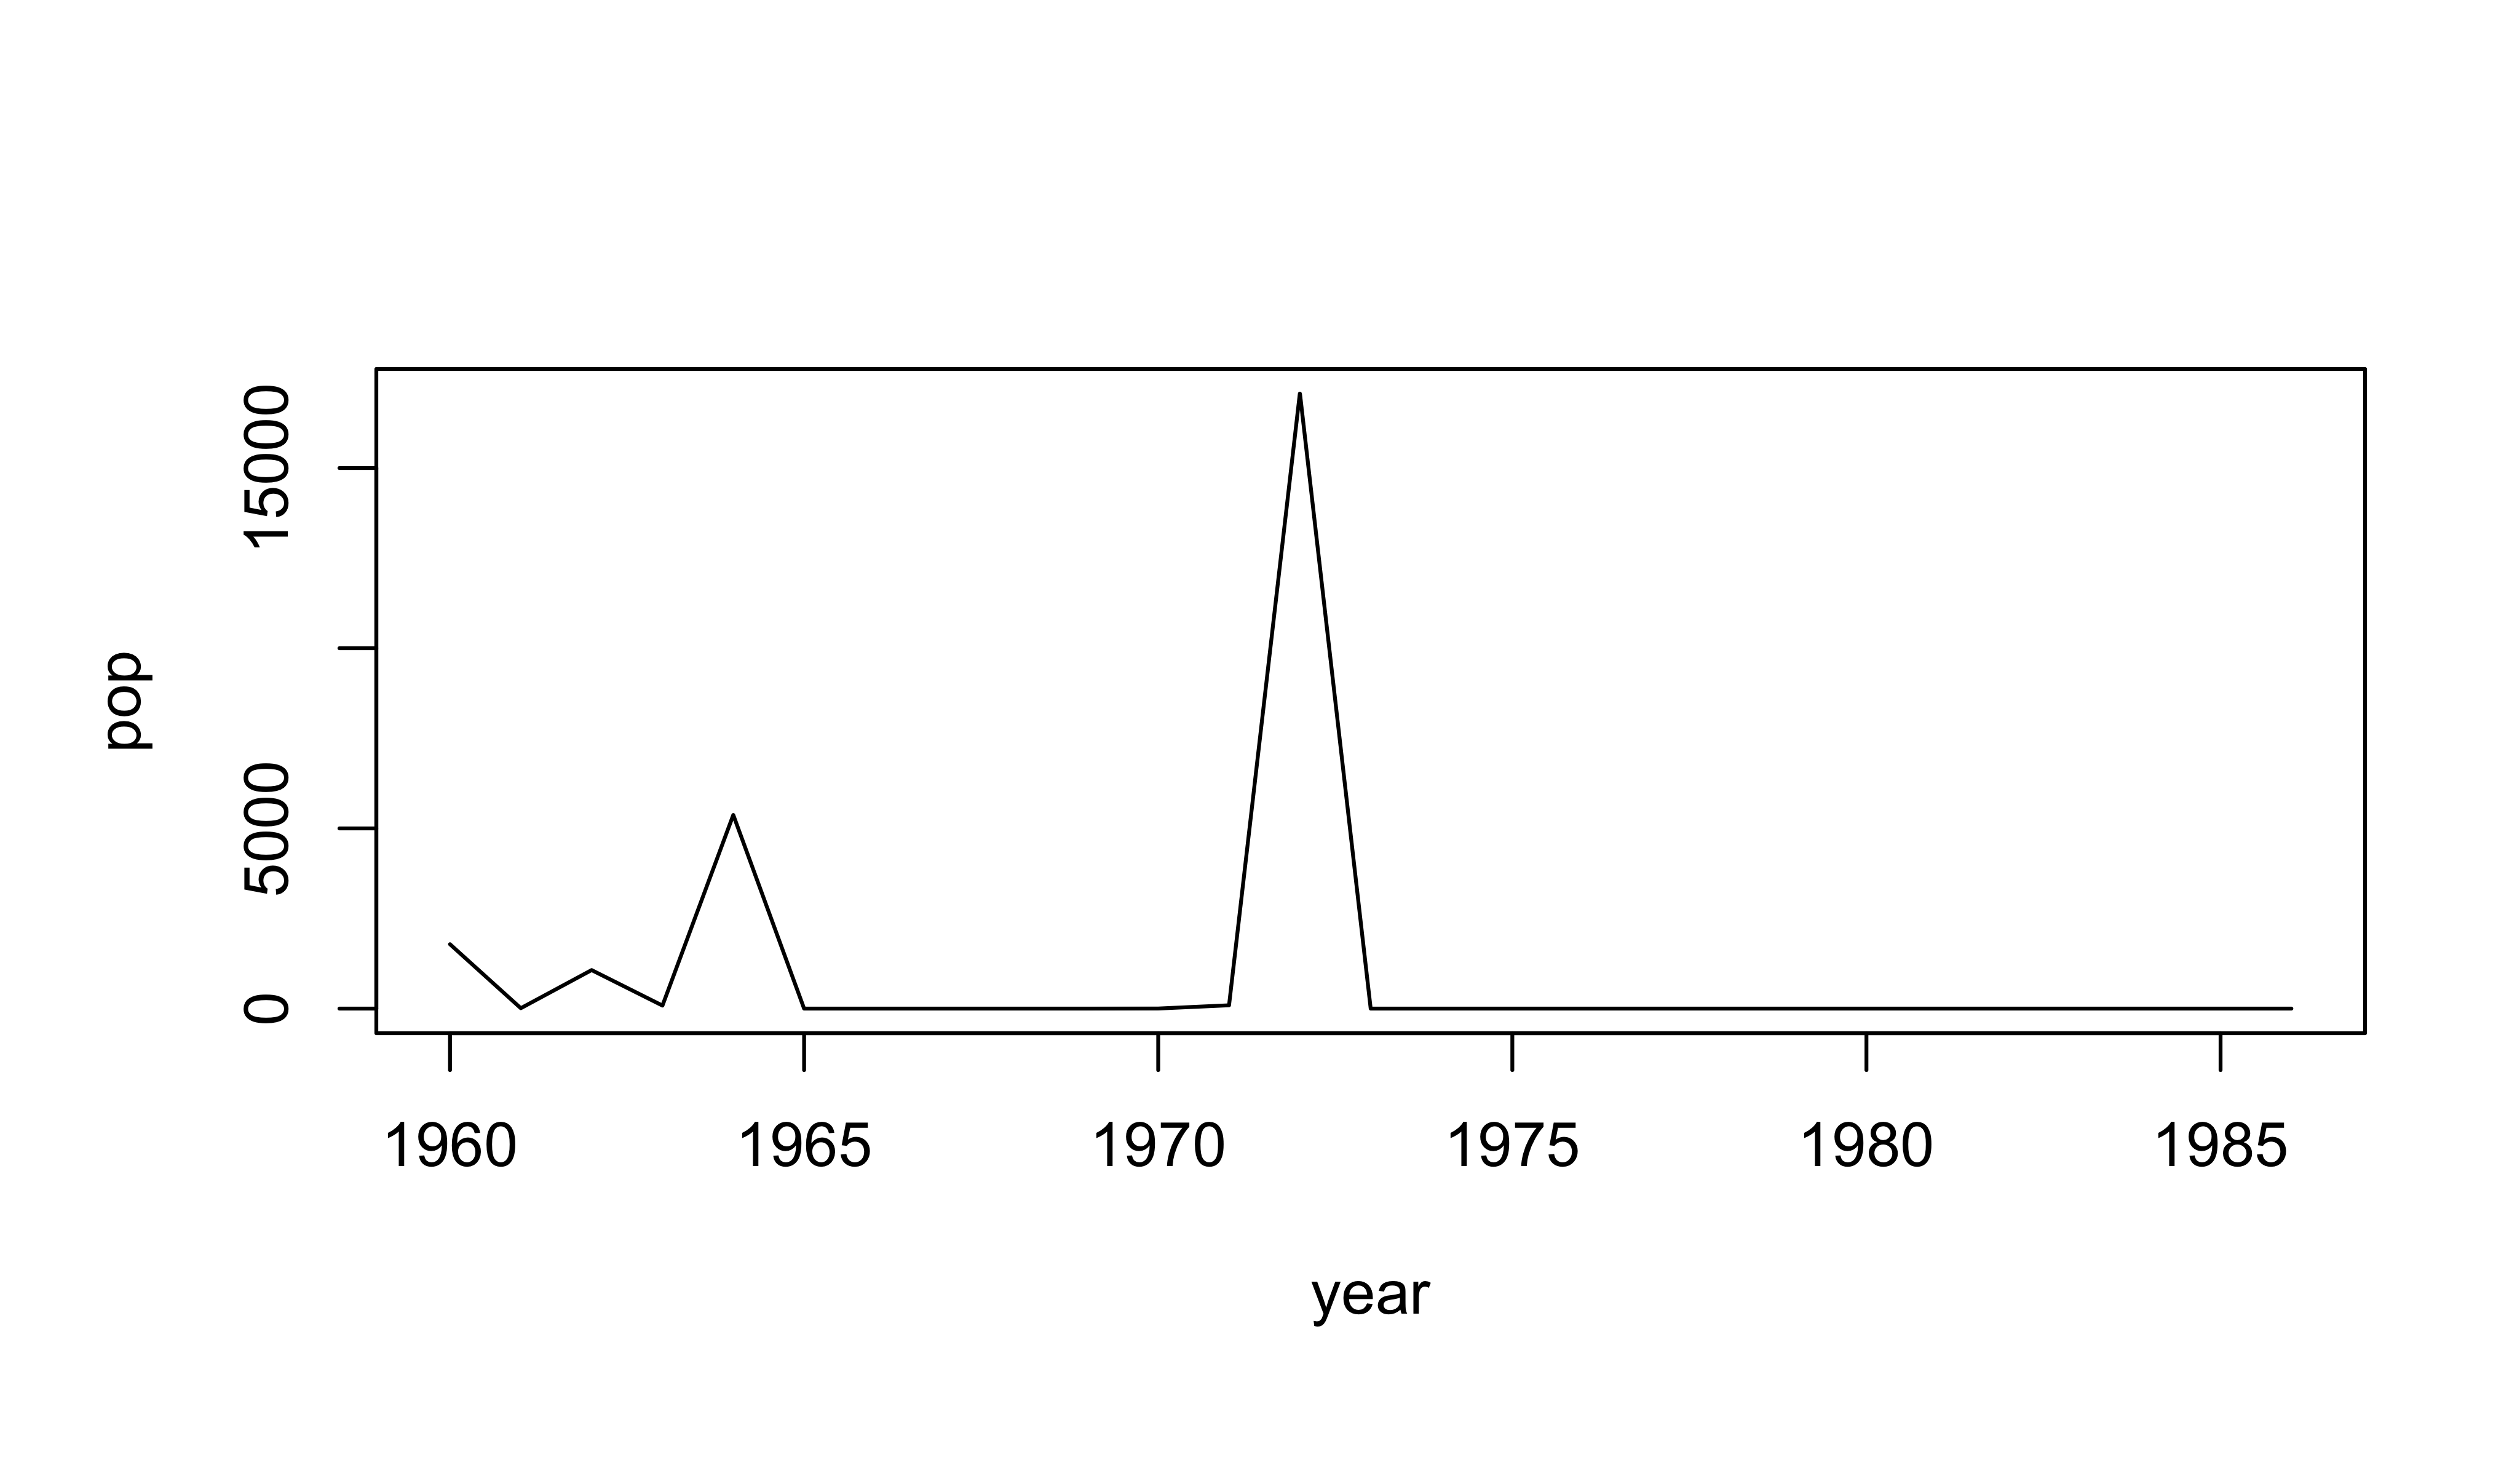
\includegraphics{tmp//figure/unnamed-chunk-6-1.png}
\end{center}
\end{frame}

\begin{frame}[fragile]{The SEIR model}
\phantomsection\label{the-seir-model}
Below is a diagram of the so-called SEIR model. This differs from the
SIR model in that infected individuals must pass a period of latency
before becoming infectious.

\begin{center}
    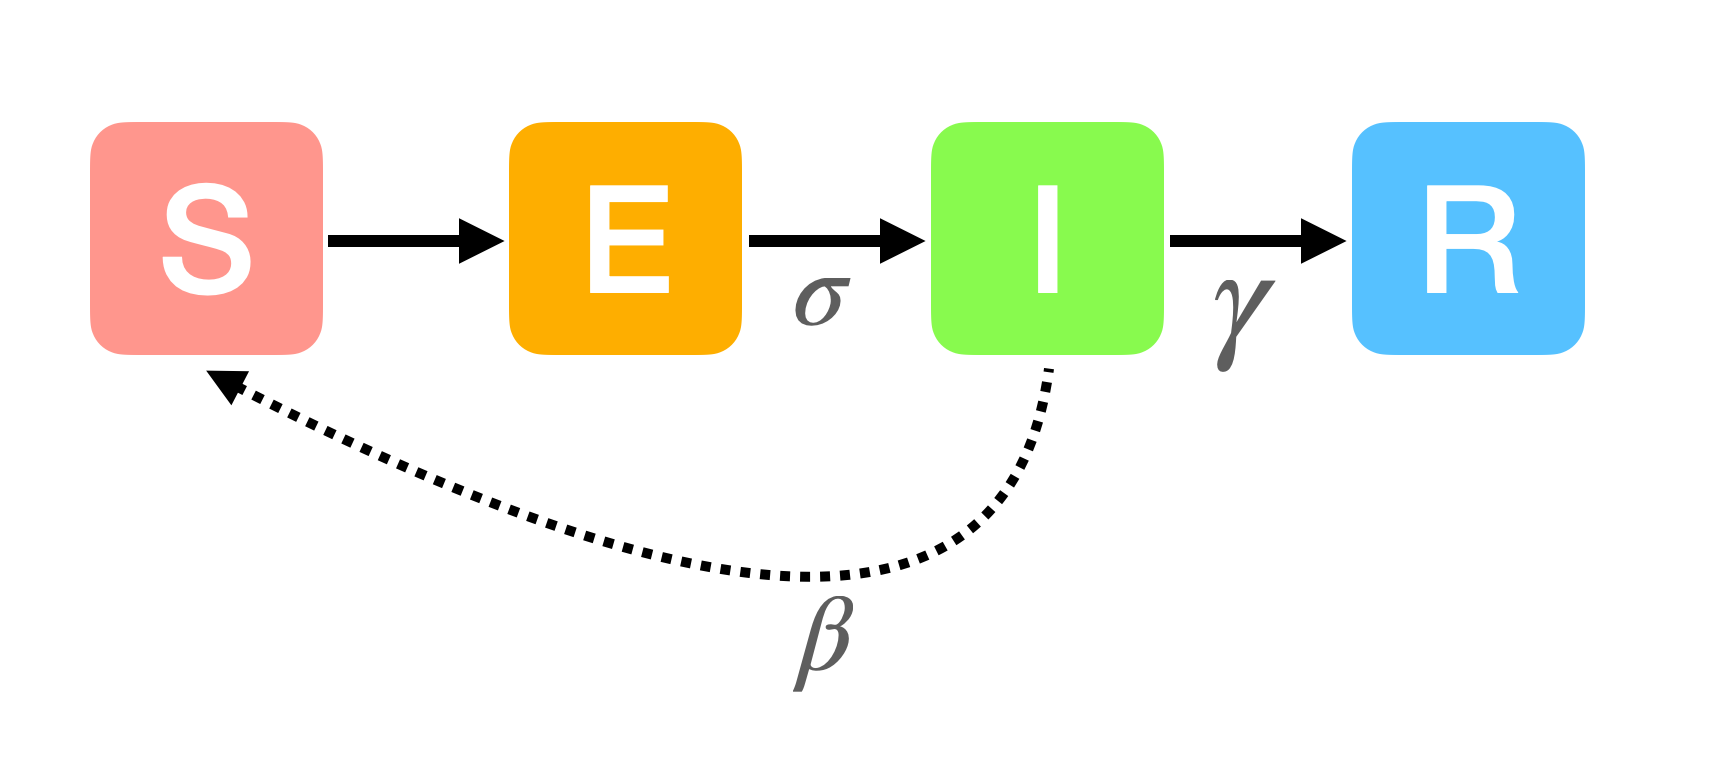
\includegraphics[height=4cm]{../graphics/SEIR model.png}
  \end{center}

Modify the codes above to construct a \texttt{pomp} object containing
the Consett measles data and an SEIR model. Perform simulations as above
and adjust parameters to get a sense of whether improvement is possible
by including a latent period.
\end{frame}

\begin{frame}[fragile,allowframebreaks]{Worked solutions: The SEIR
model}
\phantomsection\label{worked-solutions-the-seir-model}
The existing code may be modified as follows:

\begin{Shaded}
\begin{Highlighting}[]
\NormalTok{seir\_step }\OtherTok{\textless{}{-}} \FunctionTok{Csnippet}\NormalTok{(}\StringTok{"}
\StringTok{  double dN\_SE = rbinom(S,1{-}exp({-}Beta*I/N*dt));}
\StringTok{  double dN\_EI = rbinom(E,1{-}exp({-}mu\_EI*dt));}
\StringTok{  double dN\_IR = rbinom(I,1{-}exp({-}Gamma*dt));}
\StringTok{  S {-}= dN\_SE;}
\StringTok{  E += dN\_SE {-} dN\_EI;}
\StringTok{  I += dN\_EI {-} dN\_IR;}
\StringTok{  R += dN\_IR;}
\StringTok{  H += dN\_IR;}
\StringTok{"}\NormalTok{)}
\end{Highlighting}
\end{Shaded}

\begin{Shaded}
\begin{Highlighting}[]
\NormalTok{seir\_init }\OtherTok{\textless{}{-}} \FunctionTok{Csnippet}\NormalTok{(}\StringTok{"}
\StringTok{  S = nearbyint(Eta*N);}
\StringTok{  E = 0;}
\StringTok{  I = 1;}
\StringTok{  R = nearbyint((1{-}Eta)*N);}
\StringTok{  H = 0;}
\StringTok{"}\NormalTok{)}
\NormalTok{measSIR }\SpecialCharTok{|\textgreater{}}
  \FunctionTok{pomp}\NormalTok{(}
    \AttributeTok{rprocess=}\FunctionTok{euler}\NormalTok{(seir\_step,}\AttributeTok{delta.t=}\DecValTok{1}\SpecialCharTok{/}\DecValTok{7}\NormalTok{),}
    \AttributeTok{rinit=}\NormalTok{seir\_init,}
    \AttributeTok{paramnames=}\FunctionTok{c}\NormalTok{(}\StringTok{"N"}\NormalTok{,}\StringTok{"Beta"}\NormalTok{,}\StringTok{"mu\_EI"}\NormalTok{,}\StringTok{"Gamma"}\NormalTok{,}\StringTok{"Rho"}\NormalTok{,}\StringTok{"Eta"}\NormalTok{),}
    \AttributeTok{statenames=}\FunctionTok{c}\NormalTok{(}\StringTok{"S"}\NormalTok{,}\StringTok{"E"}\NormalTok{,}\StringTok{"I"}\NormalTok{,}\StringTok{"R"}\NormalTok{,}\StringTok{"H"}\NormalTok{)}
\NormalTok{  ) }\OtherTok{{-}\textgreater{}}\NormalTok{ measSEIR}
\end{Highlighting}
\end{Shaded}
\end{frame}

\begin{frame}[fragile]
Using the rough estimate that the latent period in measles is 8--10da,
we take \(\mu_{EI}\sim 0.8\)wk\textsuperscript{-1} and
\(\mu_{IR}\sim 1.3\)wk\textsuperscript{-1} (roughly the same generation
time as before).

\begin{Shaded}
\begin{Highlighting}[]
\NormalTok{measSEIR }\SpecialCharTok{|\textgreater{}}
  \FunctionTok{simulate}\NormalTok{(}\AttributeTok{params=}\FunctionTok{c}\NormalTok{(}\AttributeTok{Beta=}\DecValTok{30}\NormalTok{,}\AttributeTok{mu\_EI=}\FloatTok{0.8}\NormalTok{,}\AttributeTok{Gamma=}\FloatTok{1.3}\NormalTok{,}
                    \AttributeTok{Rho=}\FloatTok{0.5}\NormalTok{,}\AttributeTok{k=}\DecValTok{10}\NormalTok{,}\AttributeTok{Eta=}\FloatTok{0.06}\NormalTok{,}\AttributeTok{N=}\DecValTok{38000}\NormalTok{),}
    \AttributeTok{nsim=}\DecValTok{20}\NormalTok{,}\AttributeTok{format=}\StringTok{"data.frame"}\NormalTok{,}\AttributeTok{include.data=}\ConstantTok{TRUE}\NormalTok{) }\SpecialCharTok{|\textgreater{}}
  \FunctionTok{ggplot}\NormalTok{(}\FunctionTok{aes}\NormalTok{(}\AttributeTok{x=}\NormalTok{week,}\AttributeTok{y=}\NormalTok{reports,}\AttributeTok{group=}\NormalTok{.id,}\AttributeTok{color=}\NormalTok{.id}\SpecialCharTok{==}\StringTok{"data"}\NormalTok{))}\SpecialCharTok{+}
  \FunctionTok{geom\_line}\NormalTok{() }\SpecialCharTok{+} \FunctionTok{guides}\NormalTok{(}\AttributeTok{color=}\StringTok{"none"}\NormalTok{)}
\end{Highlighting}
\end{Shaded}

\begin{center}
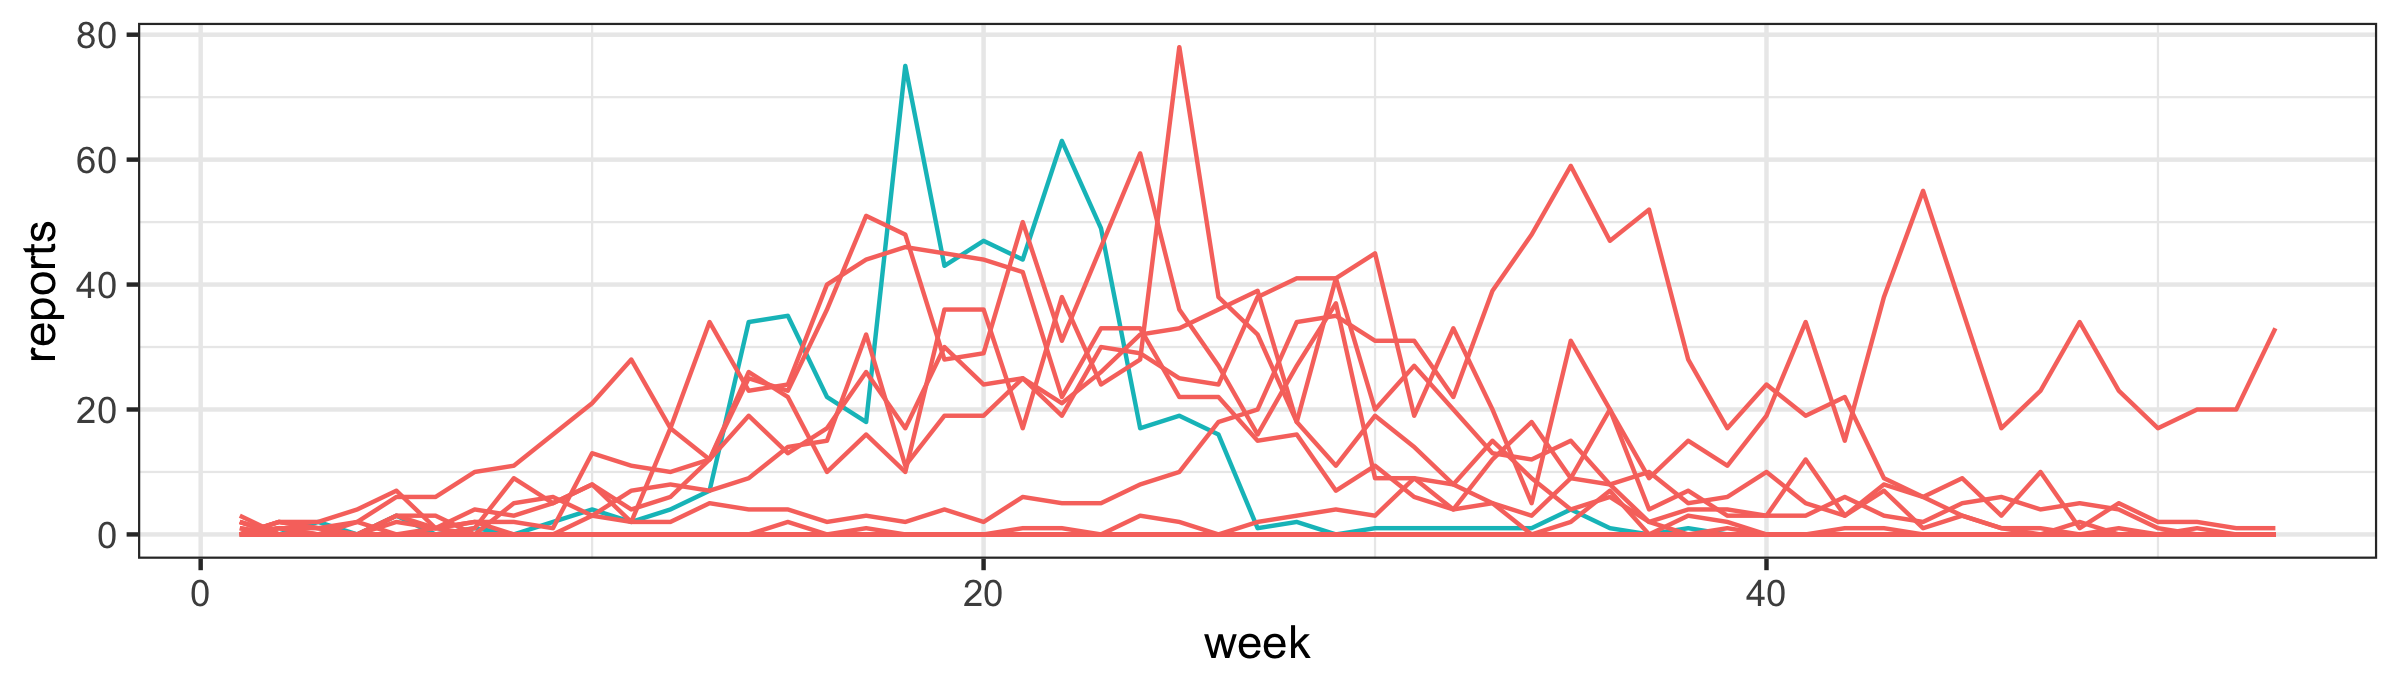
\includegraphics{tmp//figure/unnamed-chunk-9-1.png}
\end{center}
\end{frame}

\begin{frame}[fragile]
Again one can increase the force of infection:

\begin{Shaded}
\begin{Highlighting}[]
\NormalTok{measSEIR }\SpecialCharTok{|\textgreater{}} 
  \FunctionTok{simulate}\NormalTok{(}\AttributeTok{params=}\FunctionTok{c}\NormalTok{(}\AttributeTok{Beta=}\DecValTok{40}\NormalTok{,}\AttributeTok{mu\_EI=}\FloatTok{0.8}\NormalTok{,}\AttributeTok{Gamma=}\FloatTok{1.3}\NormalTok{,}
                    \AttributeTok{Rho=}\FloatTok{0.5}\NormalTok{,}\AttributeTok{k=}\DecValTok{10}\NormalTok{,}\AttributeTok{Eta=}\FloatTok{0.06}\NormalTok{,}\AttributeTok{N=}\DecValTok{38000}\NormalTok{),}
  \AttributeTok{nsim=}\DecValTok{20}\NormalTok{,}\AttributeTok{format=}\StringTok{"data.frame"}\NormalTok{,}\AttributeTok{include.data=}\ConstantTok{TRUE}\NormalTok{) }\SpecialCharTok{|\textgreater{}}
  \FunctionTok{ggplot}\NormalTok{(}\FunctionTok{aes}\NormalTok{(}\AttributeTok{x=}\NormalTok{week,}\AttributeTok{y=}\NormalTok{reports,}\AttributeTok{group=}\NormalTok{.id,}\AttributeTok{color=}\NormalTok{.id}\SpecialCharTok{==}\StringTok{"data"}\NormalTok{))}\SpecialCharTok{+}
  \FunctionTok{geom\_line}\NormalTok{()}\SpecialCharTok{+}
  \FunctionTok{guides}\NormalTok{(}\AttributeTok{color=}\StringTok{"none"}\NormalTok{)}
\end{Highlighting}
\end{Shaded}

\begin{center}
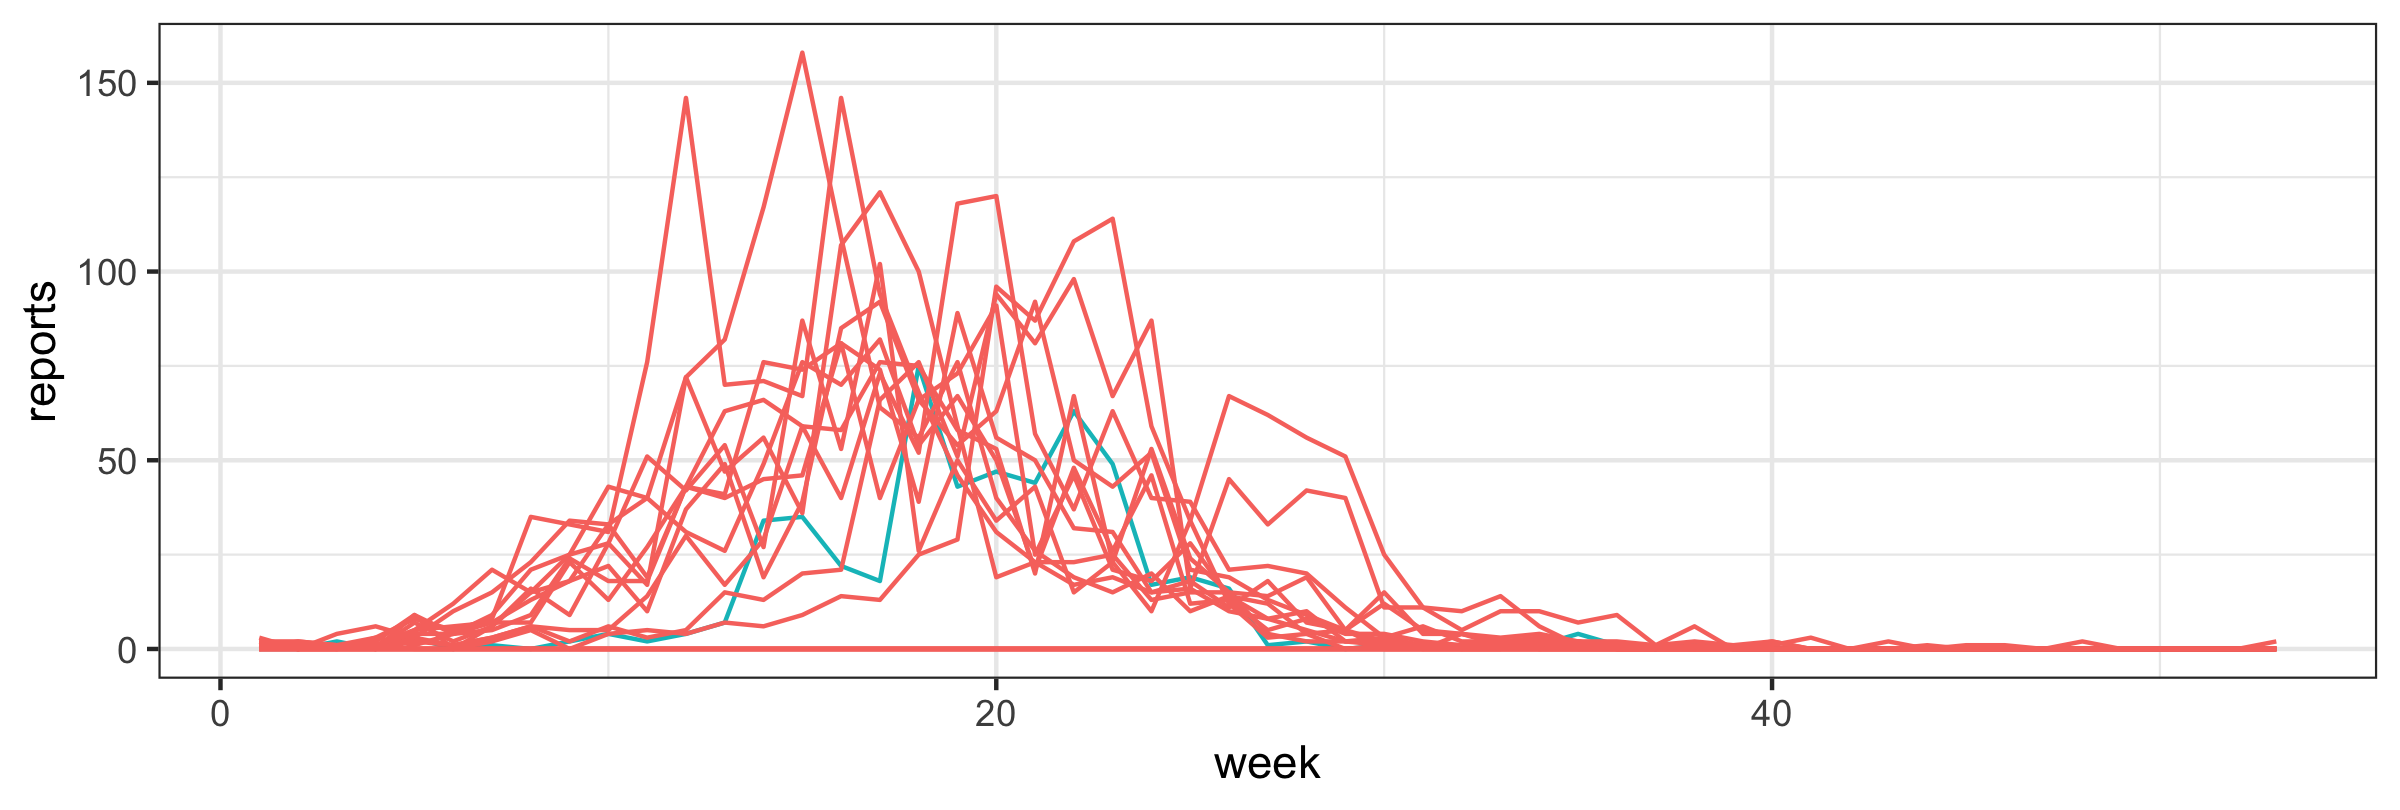
\includegraphics{tmp//figure/unnamed-chunk-10-1.png}
\end{center}
\end{frame}

\section{References}\label{references}

\begin{frame}[allowframebreaks]{References}
\phantomsection\label{references-1}
\phantomsection\label{refs}
\begin{CSLReferences}{1}{0}
\bibitem[\citeproctext]{ref-Anderson1991}
Anderson, R. M., and R. M. May. 1991. \emph{Infectious Diseases of
Humans}. Oxford: Oxford Univesity Press.

\bibitem[\citeproctext]{ref-Breto2009}
Bretó, Carles, Daihai He, Edward L. Ionides, and Aaron A. King. 2009.
{``Time Series Analysis via Mechanistic Models.''} \emph{Ann Appl Stat}
3 (1): 319--48. \url{https://doi.org/10.1214/08-AOAS201}.

\end{CSLReferences}
\end{frame}

\begin{frame}[fragile]{License, acknowledgments, and links}
\phantomsection\label{license-acknowledgments-and-links}
\begin{itemize}
\item
  This lesson is prepared for the
  \href{https://kingaa.github.io/sbied/}{Simulation-based Inference for
  Epidemiological Dynamics} module at the Summer Institute in Statistics
  and Modeling in Infectious Diseases,
  \href{https://www.biostat.washington.edu/suminst/sismid}{SISMID}.
\item
  The materials build on \href{../acknowledge.html}{previous versions of
  this course and related courses}.
\item
  Licensed under the
  \href{https://creativecommons.org/licenses/by-nc/4.0/}{Creative
  Commons Attribution-NonCommercial license}. Please share and remix
  non-commercially, mentioning its origin.
  
\includegraphics[height=12pt]{../graphics/cc-by-nc}
\item
  Produced with R version 4.4.0 and pomp version 5.9.
\item
  Compiled on 2024-06-16.
\end{itemize}

\href{index.html}{Back to Lesson}

\href{main.R}{\texttt{R} codes for this lesson}
\end{frame}



\end{document}
